\documentclass[11pt]{book}
%\usepackage[subpreambles=true]{standalone}
\usepackage[spanish]{babel}
\usepackage{comfortaa}
\usepackage[T1]{fontenc}
\usepackage[utf8x]{inputenc}
\usepackage[
letterpaper,
left=1in, 
right=1in, 
top=1in,
bottom=1in,
headheight=10mm,% Set \headheight to 10mm
]{geometry} % Custom margins
\usepackage{float}
\usepackage[colorlinks = true, linkcolor = colorrds]{hyperref}
\usepackage{bookmark}
\usepackage{fancyhdr}
\usepackage{color, colortbl}
\usepackage[dvipsnames,table]{xcolor} % Required for custom color
\usepackage{graphicx}
\usepackage{tabularx}
\usepackage{multicol,multirow}
\usepackage{newclude}
\usepackage{tabto}
\usepackage{remreset}
\usepackage[inline]{enumitem}
\usepackage{xparse}
\usepackage{wrapfig}
\usepackage{caption,capt-of}
\usepackage{amssymb,amsmath}
\usepackage{tikz}
\usepackage{etoolbox}
\usepackage{pdflscape}
%\usepackage{pdfpages}
\usepackage[explicit]{titlesec}
\usepackage{subfiles} % Best loaded last in the preamble
\input{insbox}
\makeatletter
\@removefromreset{section}{chapter}
\makeatother
\addto\captionsspanish{\renewcommand{\chaptername}{Unidad}}
\renewcommand{\thechapter}{\arabic{chapter}}
\renewcommand{\thesection}{S\arabic{section}}
\renewcommand{\thesubsection}{L\arabic{subsection}}
\newcommand*\chapterlabel{}
\titleformat{\chapter}
{\gdef\chapterlabel{}
    \comfortaa\Huge\bfseries
}
{\gdef\chapterlabel{\chaptername \ \thechapter}}{0pt}
{\begin{tikzpicture}[remember picture,overlay]
        \node[yshift=-2cm] at (current page.north west)
        {\begin{tikzpicture}[remember picture, overlay]
                \draw[draw=none,fill=teal] (0,0) rectangle
                (\paperwidth,2cm);
                \node[anchor=east,xshift=.9\paperwidth,rectangle,
                    rounded corners=5pt,inner xsep=20pt,inner ysep=5pt,
                    blur shadow={shadow blur steps=50,shadow blur extra rounding=5pt},
                    fill=brown]
                {\color{CadetBlue!20}\textbf{\chapterlabel#1}};
            \end{tikzpicture}
        };
    \end{tikzpicture}
}
\titlespacing*{\chapter}{0pt}{50pt}{-60pt}

\makeatletter
\@removefromreset{section}{chapter}
\makeatother
\addto\captionsspanish{\renewcommand{\chaptername}{Unidad}}
\renewcommand{\thechapter}{\arabic{chapter}}
\renewcommand{\thesection}{S\arabic{section}}
\renewcommand{\thesubsection}{L\arabic{subsection}}
\newcommand*\sectionlabel{}
\titleformat{\section}
{\gdef\sectionlabel{}
    \comfortaa\large\bfseries
}
{\gdef\sectionlabel{\thesection \ }}{0pt}
{\begin{tikzpicture}[remember picture,overlay]
        \node[yshift=-1.5cm] at (current page.north west)
        {\begin{tikzpicture}[remember picture, overlay]
                \draw[draw=none,fill=colorrds!30,
                    %shade,
                    rounded corners=5pt,
                    blur shadow={shadow blur steps=10,shadow blur extra rounding=10pt},
                    xshift=5mm,
                ] (0,0) rectangle
                (\paperwidth-10mm,2cm);
                \node[
                    anchor=west,
                    xshift=0.1\paperwidth,
                    rectangle,
                    %shade,
                    rounded corners=5pt,
                    inner sep=8pt,
                    fill=olive!50,
                    %drop shadow={fill=black, opacity=1},
                ]
                {\color{colorrds}\sectionlabel#1};
                % \node[anchor=east,xshift=.9\paperwidth,rectangle,
                %     rounded corners=10pt,inner sep=11pt,
                %     fill=blue!35]
                % {\color{green}\sectionlabel};
            \end{tikzpicture}
        };
    \end{tikzpicture}
}
\titlespacing*{\section}{0pt}{50pt}{0pt}
\usepackage[many]{tcolorbox}
% \usepackage{mathspec} 			    % for FONTS
% \usepackage{setspace}               % for LINE SPACING
% \setmainfont{Noto Sans}[
%     Kerning = On,
%     Mapping = tex-text,
%     Numbers = Uppercase,
%     BoldFont = Noto Sans SemiBold
% ]                           % setting the font as Noto Sans
% \setlength\parindent{0pt}   % killing indentation for all the text
% \setstretch{1.3}            % setting line spacing to 1.3
% \setlength\columnsep{0.25in} % setting length of column separator
% \pagestyle{empty}           % setting pagestyle to be empty


\definecolor{main}{HTML}{5989cf}    % setting main color to be used
\definecolor{sub}{HTML}{cde4ff}     % setting sub color to be used

\tcbset{
    sharp corners,
    colback = white,
    before skip = 0.2cm,    % add extra space before the box
    after skip = 0.5cm      % add extra space after the box
}                           % setting global options for tcolorbox


\newtcolorbox{bA}{
    %sharpish corners, % b
    enhanced,
    %colback = sub, % background color
    boxrule = 0.2pt,  % no borders
    %borderline = {1pt}{1pt}{black!35}, % add "dashed" for dashed line
    %fontupper = \bf\color{black}, % font color
    %colframe = main % frame color
    rounded corners,
    %arc = 5pt,   % corners roundness
    fuzzy shadow = {2pt}{-4pt}{-1pt}{1pt}{black!35}, % {xshift}{yshift}{offset}{step}{options} 
    %toprule = 3pt, % top rule weight
    %bottomrule = 3pt % bottom rule weight
}
% You can copy any following box you like to your code.
\newtcolorbox{boxA}{
    fontupper = \bf,
    boxrule = 1.5pt,
    colframe = black % frame color
}

\newtcolorbox{boxB}{
    fontupper = \bf\color{main}, % font color
    boxrule = 1.5pt,
    colframe = main,
    rounded corners,
    arc = 5pt   % corners roundness
}

\newtcolorbox{boxC}{
    colback = sub, % background color
    boxrule = 0pt  % no borders
}

\newtcolorbox{boxD}{
    colback = sub,
    colframe = main,
    boxrule = 0pt,
    toprule = 3pt, % top rule weight
    bottomrule = 3pt % bottom rule weight
}

\newtcolorbox{boxE}{
    enhanced, % for a fancier setting,
    boxrule = 0pt, % clearing the default rule
    borderline = {0.75pt}{0pt}{main}, % outer line
    borderline = {0.75pt}{2pt}{sub} % inner line
}

\newtcolorbox{boxF}{
    colback = sub,
    enhanced,
    boxrule = 1.5pt,
    colframe = white, % making the base for dash line
    borderline = {1.5pt}{0pt}{main, dashed} % add "dashed" for dashed line
}

\newtcolorbox{boxG}{
    enhanced,
    boxrule = 0pt,
    colback = sub,
    borderline west = {1pt}{0pt}{main},
    borderline west = {0.75pt}{2pt}{main},
    borderline east = {1pt}{0pt}{main},
    borderline east = {0.75pt}{2pt}{main}
}

\newtcolorbox{boxH}{
    colback = colorrds!10,
    colframe = colorrds,
    boxrule = 0pt,
    leftrule = 6pt % left rule weight
}

\newtcolorbox{boxI}{
    colback = sub,
    colframe = main,
    boxrule = 0pt,
    toprule = 6pt % top rule weight
}

\newtcolorbox{boxJ}{
    sharpish corners, % better drop shadow
    colback = sub,
    colframe = main,
    boxrule = 0pt,
    toprule = 4.5pt, % top rule weight
    enhanced,
    fuzzy shadow = {0pt}{-2pt}{-0.5pt}{0.5pt}{black!35} % {xshift}{yshift}{offset}{step}{options} 
}

\newtcolorbox{boxK}{
    sharpish corners, % better drop shadow
    boxrule = 0pt,
    toprule = 4.5pt, % top rule weight
    enhanced,
    fuzzy shadow = {0pt}{-4pt}{-1pt}{1pt}{black!35} % {xshift}{yshift}{offset}{step}{options} 
}

\newtcolorbox{boxL}{
    fontupper = \color{main},
    rounded corners,
    arc = 6pt,
    colback = sub,
    colframe = main!50,
    boxrule = 0pt,
    bottomrule = 4.5pt
}

\newtcolorbox{boxM}{
    fontupper = \color{white},
    rounded corners,
    arc = 6pt,
    colback = main!80,
    colframe = main,
    boxrule = 0pt,
    bottomrule = 4.5pt,
    enhanced,
    fuzzy shadow = {0pt}{-3pt}{-0.5pt}{0.5pt}{black!35}
}
% \documentclass[tikz,border=40mm]{standalone}
% \usetikzlibrary{shapes,calc}
% \usepackage{anyfontsize}
%\usepackage{mathptmx}
%\begin{document}
\newcommand{\ElemLabel}[4]{
    \begin{minipage}{2.2cm}
        \centering
        {{\fontsize{13}{13}\selectfont\bfseries #1} \hfill {\fontsize{12}{12}\selectfont #2}}\\[1ex]
        {\fontsize{36}{36}\selectfont \bfseries #3}\\[2ex]
        {\fontsize{13}{13}\selectfont  \sffamily #4}
    \end{minipage}
}

\newcommand{\NaturalElem}[4]{\ElemLabel{#1}{#2}{#3}{#4}}

\newcommand{\SyntheticElem}[4]{\ElemLabel{#1}{#2}{\color{gray}#3}{\color{gray}#4}}

\newcommand{\TablaPeriodica}[1][0.55]{
    \begin{tikzpicture}[font=\normalfont,scale=#1, transform shape]

        % Fill Color Styles
        \tikzstyle{ElementFill} = [fill=gray!40]
        \tikzstyle{AlkaliMetalFill} = [fill=RoyalPurple!40]
        \tikzstyle{AlkalineEarthMetalFill} = [fill=RoyalBlue!40]
        \tikzstyle{MetalFill} = [fill=SkyBlue!40]
        \tikzstyle{MetalloidFill} = [fill=LimeGreen!55]
        \tikzstyle{NonmetalFill} = [fill=Orange!55]
        \tikzstyle{HalogenFill} = [fill=BrickRed!55]
        \tikzstyle{NobleGasFill} = [fill=Goldenrod!40]
        \tikzstyle{LanthanideActinideFill} = [fill=teal!40]

        % Element Styles
        \tikzstyle{Element} = [ElementFill,
        minimum width=2.5cm, minimum height=2.5cm, node distance=2.75cm]
        \tikzstyle{AlkaliMetal} = [Element, AlkaliMetalFill]
        \tikzstyle{AlkalineEarthMetal} = [Element, AlkalineEarthMetalFill]
        \tikzstyle{Metal} = [Element, MetalFill]
        \tikzstyle{Metalloid} = [Element, MetalloidFill]
        \tikzstyle{Nonmetal} = [Element, NonmetalFill]
        \tikzstyle{Halogen} = [Element, HalogenFill]
        \tikzstyle{NobleGas} = [Element, NobleGasFill]
        \tikzstyle{LanthanideActinide} = [Element, LanthanideActinideFill]
        \tikzstyle{PeriodLabel} = [font={\sffamily\LARGE}, node distance=2.0cm]
        \tikzstyle{GroupLabel} = [font={\sffamily\LARGE}, minimum width=2.75cm, node distance=2.0cm]

        % Group 1 - IA
        \node[Element] (H) {\NaturalElem{1} {1.0079}{H}{Hidr\'ogeno}};
        \node[below of=H, AlkaliMetal] (Li) {\NaturalElem{3}{6.941}{Li}{Litio}};
        \node[below of=Li, AlkaliMetal] (Na) {\NaturalElem{11}{22.990}{Na}{Sodio}};
        \node[below of=Na, AlkaliMetal] (K) {\NaturalElem{19}{39.098}{K}{Potasio}};
        \node[below of=K, AlkaliMetal] (Rb) {\NaturalElem{37}{85.468}{Rb}{Rubidio}};
        \node[below of=Rb, AlkaliMetal] (Cs) {\NaturalElem{55}{132.91}{Cs}{Cesio}};
        \node[below of=Cs, AlkaliMetal] (Fr) {\NaturalElem{87}{223}{Fr}{Francio}};

        % Group 2 - IIA
        \node[right of=Li, AlkalineEarthMetal] (Be) {\NaturalElem{4}{9.0122}{Be}{Berilio}};
        \node[below of=Be, AlkalineEarthMetal] (Mg) {\NaturalElem{12}{24.305}{Mg}{Magnesio}};
        \node[below of=Mg, AlkalineEarthMetal] (Ca) {\NaturalElem{20}{40.078}{Ca}{Calcio}};
        \node[below of=Ca, AlkalineEarthMetal] (Sr) {\NaturalElem{38}{87.62}{Sr}{Stroncio}};
        \node[below of=Sr, AlkalineEarthMetal] (Ba) {\NaturalElem{56}{137.33}{Ba}{Bario}};
        \node[below of=Ba, AlkalineEarthMetal] (Ra) {\NaturalElem{88}{226}{Ra}{Radio}};

        % Group 3 - IIIB
        \node[right of=Ca, Metal] (Sc) {\NaturalElem{21}{44.956}{Sc}{Escandio}};
        \node[below of=Sc, Metal] (Y) {\NaturalElem{39}{88.906}{Y}{Itrio}};
        \node[below of=Y, LanthanideActinide] (LaLu) {\NaturalElem{57-71}{}{*}{Lant\'anido}};
        \node[below of=LaLu, LanthanideActinide] (AcLr) {\NaturalElem{89-103}{}{**}{Act\'inido}};

        % Group 4 - IVB
        \node[right of=Sc, Metal] (Ti) {\NaturalElem{22}{47.867}{Ti}{Titanio}};
        \node[below of=Ti, Metal] (Zr) {\NaturalElem{40}{91.224}{Zr}{Circonio}};
        \node[below of=Zr, Metal] (Hf) {\NaturalElem{72}{178.49}{Hf}{Hafnio}};
        \node[below of=Hf, Metal] (Rf) {\SyntheticElem{104}{261}{Rf}{Rutherfordio}};

        % Group 5 - VB
        \node[right of=Ti, Metal] (V) {\NaturalElem{23}{50.942}{V}{Vanadio}};
        \node[below of=V, Metal] (Nb) {\NaturalElem{41}{92.906}{Nb}{Niobio}};
        \node[below of=Nb, Metal] (Ta) {\NaturalElem{73}{180.95}{Ta}{Tantalo}};
        \node[below of=Ta, Metal] (Db) {\SyntheticElem{105}{262}{Db}{Dubnio}};

        % Group 6 - VIB
        \node[right of=V, Metal] (Cr) {\NaturalElem{24}{51.996}{Cr}{Cromo}};
        \node[below of=Cr, Metal] (Mo) {\NaturalElem{42}{95.94}{Mo}{Molybdeno}};
        \node[below of=Mo, Metal] (W) {\NaturalElem{74}{183.84}{W}{Tungstenio}};
        \node[below of=W, Metal] (Sg) {\SyntheticElem{106}{266}{Sg}{Seaborgio}};

        % Group 7 - VIIB
        \node[right of=Cr, Metal] (Mn) {\NaturalElem{25}{54.938}{Mn}{Manganeso}};
        \node[below of=Mn, Metal] (Tc) {\NaturalElem{43}{96}{Tc}{Tecnecio}};
        \node[below of=Tc, Metal] (Re) {\NaturalElem{75}{186.21}{Re}{Renio}};
        \node[below of=Re, Metal] (Bh) {\SyntheticElem{107}{264}{Bh}{Bohrio}};

        % Group 8 - VIIIB
        \node[right of=Mn, Metal] (Fe) {\NaturalElem{26}{55.845}{Fe}{Hierro}};
        \node[below of=Fe, Metal] (Ru) {\NaturalElem{44}{101.07}{Ru}{Ruthenio}};
        \node[below of=Ru, Metal] (Os) {\NaturalElem{76}{190.23}{Os}{Osmio}};
        \node[below of=Os, Metal] (Hs) {\SyntheticElem{108}{277}{Hs}{Hassio}};

        % Group 9 - VIIIB
        \node[right of=Fe, Metal] (Co) {\NaturalElem{27}{58.933}{Co}{Cobalto}};
        \node[below of=Co, Metal] (Rh) {\NaturalElem{45}{102.91}{Rh}{Rodio}};
        \node[below of=Rh, Metal] (Ir) {\NaturalElem{77}{192.22}{Ir}{Iridio}};
        \node[below of=Ir, Metal] (Mt) {\SyntheticElem{109}{268}{Mt}{Meitnerio}};

        % Group 10 - VIIIB
        \node[right of=Co, Metal] (Ni) {\NaturalElem{28}{58.693}{Ni}{Niquel}};
        \node[below of=Ni, Metal] (Pd) {\NaturalElem{46}{106.42}{Pd}{Paladio}};
        \node[below of=Pd, Metal] (Pt) {\NaturalElem{78}{195.08}{Pt}{Platino}};
        \node[below of=Pt, Metal] (Ds) {\SyntheticElem{110}{281}{Ds}{Darmstadtio}};

        % Group 11 - IB
        \node[right of=Ni, Metal] (Cu) {\NaturalElem{29}{63.546}{Cu}{Cobre}};
        \node[below of=Cu, Metal] (Ag) {\NaturalElem{47}{107.87}{Ag}{Plata}};
        \node[below of=Ag, Metal] (Au) {\NaturalElem{79}{196.97}{Au}{Oro}};
        \node[below of=Au, Metal] (Rg) {\SyntheticElem{111}{280}{Rg}{Roentgenio}};

        % Group 12 - IIB
        \node[right of=Cu, Metal] (Zn) {\NaturalElem{30}{65.39}{Zn}{Zinc}};
        \node[below of=Zn, Metal] (Cd) {\NaturalElem{48}{112.41}{Cd}{Cadmio}};
        \node[below of=Cd, Metal] (Hg) {\NaturalElem{80}{200.59}{Hg}{Mercurio}};
        \node[below of=Hg, Metal] (Cn) {\SyntheticElem{112}{285}{Cn}{Copernicio}};

        % Group 13 - IIIA
        \node[right of=Zn, Metal] (Ga) {\NaturalElem{31}{69.723}{Ga}{Galio}};
        \node[above of=Ga, Metal] (Al) {\NaturalElem{13}{26.982}{Al}{Aluminio}};
        \node[above of=Al, Metalloid] (B) {\NaturalElem{5}{10.811}{B}{Boro}};
        \node[below of=Ga, Metal] (In) {\NaturalElem{49}{114.82}{In}{Indo}};
        \node[below of=In, Metal] (Tl) {\NaturalElem{81}{204.38}{Tl}{Talio}};
        \node[below of=Tl, Metal] (Nh) {\SyntheticElem{113}{284}{Nh}{Nihonio}};

        % Group 14 - IVA
        \node[right of=B, Nonmetal] (C) {\NaturalElem{6}{12.011}{C}{Carbono}};
        \node[below of=C, Metalloid] (Si) {\NaturalElem{14}{28.086}{Si}{Silicio}};
        \node[below of=Si, Metalloid] (Ge) {\NaturalElem{32}{72.64}{Ge}{Germanio}};
        \node[below of=Ge, Metal] (Sn) {\NaturalElem{50}{118.71}{Sn}{Esta\~no}};
        \node[below of=Sn, Metal] (Pb) {\NaturalElem{82}{207.2}{Pb}{Plomo}};
        \node[below of=Pb, Metal] (Fl) {\SyntheticElem{114}{289}{Fl}{Flerovio}};

        % Group 15 - VA
        \node[right of=C, Nonmetal] (N) {\NaturalElem{7}{14.007}{N}{Nitr\'ogeno}};
        \node[below of=N, Nonmetal] (P) {\NaturalElem{15}{30.974}{P}{F\'osforo}};
        \node[below of=P, Metalloid] (As) {\NaturalElem{33}{74.922}{As}{Ars\'enico}};
        \node[below of=As, Metalloid] (Sb) {\NaturalElem{51}{121.76}{Sb}{Antimonio}};
        \node[below of=Sb, Metal] (Bi) {\NaturalElem{83}{208.98}{Bi}{Bismuto}};
        \node[below of=Bi, Metal] (Mc) {\SyntheticElem{115}{288}{Mc}{Moscovio}};

        % Group 16 - VIA
        \node[right of=N, Nonmetal] (O) {\NaturalElem{8}{15.999}{O}{Ox\'igeno}};
        \node[below of=O, Nonmetal] (S) {\NaturalElem{16}{32.065}{S}{Az\'ufre}};
        \node[below of=S, Nonmetal] (Se) {\NaturalElem{34}{78.96}{Se}{Selenio}};
        \node[below of=Se, Metalloid] (Te) {\NaturalElem{52}{127.6}{Te}{Tellurio}};
        \node[below of=Te, Metalloid] (Po) {\NaturalElem{84}{209}{Po}{Polonio}};
        \node[below of=Po, Metal] (Lv) {\SyntheticElem{116}{293}{Lv}{Libermonio}};

        % Group 17 - VIIA
        \node[right of=O, Halogen] (F) {\NaturalElem{9}{18.998}{F}{Fluor}};
        \node[below of=F, Halogen] (Cl) {\NaturalElem{17}{35.453}{Cl}{Cloro}};
        \node[below of=Cl, Halogen] (Br) {\NaturalElem{35}{79.904}{Br}{Bromo}};
        \node[below of=Br, Halogen] (I) {\NaturalElem{53}{126.9}{I}{Yodo}};
        \node[below of=I, Halogen] (At) {\NaturalElem{85}{210}{At}{\'Astato}};
        \node[below of=At, Element] (Ts) {\SyntheticElem{117}{292}{Ts}{Teneso}};

        % Group 18 - VIIIA
        \node[right of=F, NobleGas] (Ne) {\NaturalElem{10}{20.180}{Ne}{Ne\'on}};
        \node[above of=Ne, NobleGas] (He) {\NaturalElem{2}{4.0025}{He}{Helio}};
        \node[below of=Ne, NobleGas] (Ar) {\NaturalElem{18}{39.948}{Ar}{Arg\'on}};
        \node[below of=Ar, NobleGas] (Kr) {\NaturalElem{36}{83.8}{Kr}{Kript\'on}};
        \node[below of=Kr, NobleGas] (Xe) {\NaturalElem{54}{131.29}{Xe}{Xen\'on}};
        \node[below of=Xe, NobleGas] (Rn) {\NaturalElem{86}{222}{Rn}{Rad\'on}};
        \node[below of=Rn, Nonmetal] (Og) {\SyntheticElem{118}{294}{Og}{Oganesón}};

        % Period
        \node[left of=H, PeriodLabel] (Period1) {1};
        \node[left of=Li, PeriodLabel] (Period2) {2};
        \node[left of=Na, PeriodLabel] (Period3) {3};
        \node[left of=K, PeriodLabel] (Period4) {4};
        \node[left of=Rb, PeriodLabel] (Period5) {5};
        \node[left of=Cs, PeriodLabel] (Period6) {6};
        \node[left of=Fr, PeriodLabel] (Period7) {7};

        % Group
        \node[above of=H, GroupLabel] (Group1) {1 \hfill IA};
        \node[above of=Be, GroupLabel] (Group2) {2 \hfill IIA};
        \node[above of=Sc, GroupLabel] (Group3) {3 \hfill IIIA};
        \node[above of=Ti, GroupLabel] (Group4) {4 \hfill IVB};
        \node[above of=V, GroupLabel] (Group5) {5 \hfill VB};
        \node[above of=Cr, GroupLabel] (Group6) {6 \hfill VIB};
        \node[above of=Mn, GroupLabel] (Group7) {7 \hfill VIIB};
        \node[above of=Fe, GroupLabel] (Group8) {8 \hfill VIIIB};
        \node[above of=Co, GroupLabel] (Group9) {9 \hfill VIIIB};
        \node[above of=Ni, GroupLabel] (Group10) {10 \hfill VIIIB};
        \node[above of=Cu, GroupLabel] (Group11) {11 \hfill IB};
        \node[above of=Zn, GroupLabel] (Group12) {12 \hfill IIB};
        \node[above of=B, GroupLabel] (Group13) {13 \hfill IIIA};
        \node[above of=C, GroupLabel] (Group14) {14 \hfill IVA};
        \node[above of=N, GroupLabel] (Group15) {15 \hfill VA};
        \node[above of=O, GroupLabel] (Group16) {16 \hfill VIA};
        \node[above of=F, GroupLabel] (Group17) {17 \hfill VIIA};
        \node[above of=He, GroupLabel] (Group18) {18 \hfill VIIIA};


        % Lanthanide
        \node[below of=Rf, LanthanideActinide, yshift=-1cm] (La) {\NaturalElem{57}{138.91}{La}{Lant\'anido}};
        \node[right of=La, LanthanideActinide] (Ce) {\NaturalElem{58}{140.12}{Ce}{Cerio}};
        \node[right of=Ce, LanthanideActinide] (Pr) {\NaturalElem{59}{140.91}{Pr}{Praseodymio}};
        \node[right of=Pr, LanthanideActinide] (Nd) {\NaturalElem{60}{144.24}{Nd}{Neodimio}};
        \node[right of=Nd, LanthanideActinide] (Pm) {\NaturalElem{61}{145}{Pm}{Prometio}};
        \node[right of=Pm, LanthanideActinide] (Sm) {\NaturalElem{62}{150.36}{Sm}{Samario}};
        \node[right of=Sm, LanthanideActinide] (Eu) {\NaturalElem{63}{151.96}{Eu}{Europio}};
        \node[right of=Eu, LanthanideActinide] (Gd) {\NaturalElem{64}{157.25}{Gd}{Gadolinio}};
        \node[right of=Gd, LanthanideActinide] (Tb) {\NaturalElem{65}{158.93}{Tb}{Terbio}};
        \node[right of=Tb, LanthanideActinide] (Dy) {\NaturalElem{66}{162.50}{Dy}{Disprosio}};
        \node[right of=Dy, LanthanideActinide] (Ho) {\NaturalElem{67}{164.93}{Ho}{Holmio}};
        \node[right of=Ho, LanthanideActinide] (Er) {\NaturalElem{68}{167.26}{Er}{Erbio}};
        \node[right of=Er, LanthanideActinide] (Tm) {\NaturalElem{69}{168.93}{Tm}{Tulio}};
        \node[right of=Tm, LanthanideActinide] (Yb) {\NaturalElem{70}{173.04}{Yb}{Yterbio}};
        \node[right of=Yb, LanthanideActinide] (Lu) {\NaturalElem{71}{174.97}{Lu}{Luterio}};

        % Actinide
        \node[below of=La, LanthanideActinide] (Ac) {\NaturalElem{89}{227}{Ac}{Actinio}};
        \node[right of=Ac, LanthanideActinide]              (Th) {\NaturalElem{90}{232.04}{Th}{Torio}};
        \node[right of=Th, LanthanideActinide]              (Pa) {\NaturalElem{91}{231.04}{Pa}{Protactinio}};
        \node[right of=Pa, LanthanideActinide]              (U)  {\NaturalElem{92}{238.03}{U}{Uranio}};
        \node[right of=U, LanthanideActinide]               (Np) {\SyntheticElem{93}{237}{Np}{Neptunio}};
        \node[right of=Np, LanthanideActinide]              (Pu) {\SyntheticElem{94}{244}{Pu}{Plutonio}};
        \node[right of=Pu, LanthanideActinide]              (Am) {\SyntheticElem{95}{243}{Am}{Americio}};
        \node[right of=Am, LanthanideActinide]              (Cm) {\SyntheticElem{96}{247}{Cm}{Curio}};
        \node[right of=Cm, LanthanideActinide]              (Bk) {\SyntheticElem{97}{247}{Bk}{Berkelio}};
        \node[right of=Bk, LanthanideActinide]              (Cf) {\SyntheticElem{98}{251}{Cf}{Californio}};
        \node[right of=Cf, LanthanideActinide]              (Es) {\SyntheticElem{99}{252}{Es}{Einsteinio}};
        \node[right of=Es, LanthanideActinide]              (Fm) {\SyntheticElem{100}{257}{Fm}{Fermio}};
        \node[right of=Fm, LanthanideActinide]              (Md) {\SyntheticElem{101}{258}{Md}{Mendelevio}};
        \node[right of=Md, LanthanideActinide]              (No) {\SyntheticElem{102}{259}{No}{Nobelio}};
        \node[right of=No, LanthanideActinide]              (Lr) {\SyntheticElem{103}{262}{Lr}{Lawrencio}};

        % Draw dotted lines connecting Lanthanide breakout to main table
        \draw[thick,dotted] (LaLu.north east) -- (La.north west)
        (LaLu.south west) -- (La.south west);
        % Draw dotted lines connecting Actinide breakout to main table
        \draw[thick,dotted] (AcLr.north east) -- (Ac.north west)
        (AcLr.south west) -- (Ac.south west);

        % Legend
        \fill[AlkaliMetalFill] ($(La -| Period7.west) + (0em,2em)$)
        rectangle +(2em, 2em) node[right, yshift=-2ex]  (AlkaliMetal) {\fontsize{20}{20}\selectfont \bfseries Metales Alcalinos};
        \fill[AlkalineEarthMetalFill] ($(AlkaliMetal.west) - (2em,4em)$)
        rectangle +(2em, 2em) node[right, yshift=-2ex] (AlkalineEarthMetal) {\fontsize{20}{20}\selectfont \bfseries Metales Alcalino-terreos};
        \fill[MetalFill] ($(AlkalineEarthMetal.west) - (2em,4em)$)
        rectangle +(2em, 2em) node[right, yshift=-2ex] (Metal) {\fontsize{20}{20}\selectfont \bfseries Metal};
        \fill[MetalloidFill] ($(Metal.west) - (2em,4em)$)
        rectangle +(2em, 2em) node[right, yshift=-2ex] (Metalloid) {\fontsize{20}{20}\selectfont \bfseries Metaloide};
        \fill[NonmetalFill] ($(Metalloid.west) - (2em,4em)$)
        rectangle +(2em, 2em) node[right, yshift=-2ex] (Non-metal) {\fontsize{20}{20}\selectfont \bfseries No metal};
        \fill[HalogenFill] ($(Non-metal.west) - (2em,4em)$)
        rectangle +(2em, 2em) node[right, yshift=-2ex] (Halogen) {\fontsize{20}{20}\selectfont \bfseries Hal\'ogeno};
        \fill[NobleGasFill] ($(Halogen.west) - (2em,4em)$)
        rectangle +(2em, 2em) node[right, yshift=-2ex] (NobleGas) {\fontsize{20}{20}\selectfont \bfseries Gases Nobles};
        \fill[LanthanideActinideFill] ($(NobleGas.west) - (2em,4em)$)
        rectangle +(2em, 2em) node[right, yshift=-2ex] (Lanthanide/Actinide) {\fontsize{20}{20}\selectfont \bfseries Lant\'anidos/Act\'inidos};

        \node at (Li -| V) [draw, Element, fill=white] (legend) {\NaturalElem{Z}{$A_r$}{\fontsize{36}{36}\selectfont S}{Símbolo}};
        \node[align=left,xshift=2mm] at (Li -| Cr.east) {\fontsize{20}{20}\selectfont \bfseries Negro: Naturales \\ {\fontsize{20}{20}\selectfont \bfseries\color{gray}Gris: Sint\'eticos}};
        \node[align=center] at (H -| Cr) {\fontsize{36}{6}\selectfont  \bfseries Simbología:};

        % Diagram Title
        % \node at (H.west -| Fe.north) [scale=2, font={\sffamily\Huge\bfseries}]
        % {Tabla Peri\'odica de los Elementos};

    \end{tikzpicture}
}
%\end{document}
\decimalpoint
%\captionsetup{width=.45\textwidth}
\setlength{\parindent}{0pt}
\graphicspath{{./Images}} %Setting the graphicspath
\definecolor{colorrds}{HTML}{0060A0} % Custom colour
%%% Headings and footer
\renewcommand\spanishtablename{Tabla}
\cfoot{\thepage}
\renewcommand{\headrulewidth}{0.2pt}
\renewcommand{\footrulewidth}{0.2pt}
%%%
\usetikzlibrary{
  arrows,
  positioning,
  matrix,
  calc,
  decorations.pathreplacing,
  decorations.pathmorphing,
  decorations.markings,
  decorations.text,
  shapes,
  shapes.symbols,
  backgrounds,
  shadows.blur,
  trees,
  fit,
  snakes,
  patterns,
  mindmap,
  intersections,
  calendar,
  plotmarks,
  spy,
  tikzmark}

%%%% APRENDISAJES TEXTBOX
\tikzset{
  abstractbox/.style={
    draw=black, fill=white, rectangle, 
    inner sep=15pt, style=rounded corners,
    drop shadow={fill=black, opacity=1}
  },
  abstracttitle/.style={fill=white}
}
\newcommand{\boxabstract}[2][fill=white]{
  \begin{tikzpicture}
    \node [abstractbox, #1] (box)
    {\begin{minipage}{0.9\linewidth}
        \setlength{\parindent}{0mm} % Indentar.
        \normalfont #2
      \end{minipage}};
    \node[abstracttitle, right=5pt] at (box.north west) {\textbf{Aprendizajes esperados:}};
    \node[draw=none, fit=(box)] {};
  \end{tikzpicture}
}%
%%%%%%%%%%%%%%%%%%%%%%%%
%\renewcommand{\labelenumi}{\mbox{\arabic{enumi}}}
%\%renewcommand{\labelitemi}{$\square$}

%%%%%%%%%%%%% START questions env
%Idea from https://tex.stackexchange.com/a/236668/1952
% \DeclareDocumentCommand\question{o}{%
%     \item\IfNoValueTF{#1}{}{(#1 puntos)}}
% \newenvironment{questions}[1][]{\enumerate[,#1]}{\endenumerate}
%\DeclareDocumentCommand\part{o}{%
% \item\IfNoValueTF{#1}{}{(#1 puntos)}}
% \newenvironment{parts}[1][]{\enumerate[,#1]}{\endenumerate}
% \newcommand{\part}{\item}
%%\newcommand{\choice}{\item}
% \newlist{parts}{enumerate*}{1}
% \setlist[parts,1]{label=(\alph*), itemjoin={{\quad}},leftmargin = 1cm}
% \newlist{oneparchoices}{enumerate*}{1}
% \setlist[oneparchoices,1]{label=\quad\alph*), itemjoin={{\quad}},leftmargin = 1cm}
% \newlist{choices}{itemize}{1}
% \setlist[choices,1]{label=\quad$\square$, itemjoin={{\\}},leftmargin = 1cm}
\newlist{hoptboxes}{itemize*}{1}
\setlist[hoptboxes,1]{label=\Large$\square$, font=\color{colorrds},itemjoin={{\quad}},leftmargin = 1cm}
\newlist{hoptions}{enumerate*}{1}
\setlist[hoptions,1]{label=(\alph*), font=\color{colorrds},itemjoin={{\quad}},leftmargin = 1cm}
%%%%%%%%%%%%% END questions env
\newenvironment{mybox}[3][]{%
  \begin{tikzpicture}[#1]%
    \def\myboxname{#3}%
    % good options: minimum height, minimum width
    \node [draw, inner sep=2ex,  align=justify]
      (BOXCONTENT) \bgroup\rule{0ex}{0ex}\ignorespaces
  }{%
    \egroup;
    \node [right, inner sep=3pt, fill=colorrds!75, outer sep=0pt, 
      text height=2ex, text depth=.5ex] (BOXNAME) 
      at ([shift={(-1em,5pt)}]BOXCONTENT.north west) {\myboxname};
    \fill[colorrds] (BOXNAME.north east) -- +(-1em,1em)
      -- +(-1em,0) -- cycle;
    \fill[colorrds] (BOXNAME.south west) -- +(1em,-1em)
      -- +(1em,0) -- cycle;
  \end{tikzpicture}
}
\begin{document}
\pagestyle{empty}
\newgeometry{left=0mm,top=50mm,bottom=0mm,right=0mm}
\documentclass[]{book}
\usepackage{geometry,graphicx} % Custom margins
\usepackage[spanish]{babel}
\usepackage[T1]{fontenc}
\usepackage[dvipsnames]{xcolor} % Required for custom color
\usepackage{color,colortbl}
\usepackage[utf8]{inputenc}
\usepackage{geometry} % Custom margins
\usepackage[spanish]{babel}
\usepackage{adjustbox,dashbox}
\usepackage{array}
\usepackage{tikz,pgfplots,pgfkeys}
\usepackage{forest,mathtools,siunitx}
\usepackage{amsfonts, amssymb, amsxtra, amsmath, amsbsy}
\usepackage{newclude}
\usepackage{ifthen}
\usepackage{float}
\usepackage{fancybox}
\usepackage{graphicx,tabularx}
\usepackage{multicol,multirow}
\usepackage{enumitem} % Customising the numbered lists
\usepackage{xhfill} % Making the pink block not extend beyond the margin
\usepackage{nameref} % reference the names of the sections
\usepackage{caption,capt-of}
\usepackage[normalem]{ulem} % Dashed lines in appendix
\usepackage{ragged2e} % Ragged left
\usepackage{booktabs}
\usepackage[unboxed]{cwpuzzle}
\usepackage[colorlinks = true,linkcolor = blue]{hyperref}
\usepackage{subfiles}
\usepackage{wrapfig}
\input{insbox}
\usepackage{etoolbox}
\usepackage{mwe}
\usepackage{comfortaa}
\usepackage[T1]{fontenc}
\renewcommand*\oldstylenums[1]{{\firaoldstyle #1}}
\usepackage[T1]{fontenc}
\usepackage{pythontex}
\usepackage{polynom}
\usepackage{longdivision}


\title{Actividades}
\author{Julio C. Melchor P.\thanks{{\tt julio.melchor@rafaeldiazserdan.net}}}
\date{v1.0, \today}
%\usepackage[dvipsnames]{xcolor} % Required for custom color
\usepackage{color,colortbl}
\usepackage[utf8]{inputenc}
\usepackage{geometry} % Custom margins
\usepackage[spanish]{babel}
\usepackage{adjustbox,dashbox}
\usepackage{array}
\usepackage{tikz,pgfplots,pgfkeys}
\usepackage{forest,mathtools,siunitx}
\usepackage{amsfonts, amssymb, amsxtra, amsmath, amsbsy}
\usepackage{newclude}
\usepackage{ifthen}
\usepackage{float}
\usepackage{fancybox}
\usepackage{graphicx,tabularx}
\usepackage{multicol,multirow}
\usepackage{enumitem} % Customising the numbered lists
\usepackage{xhfill} % Making the pink block not extend beyond the margin
\usepackage{nameref} % reference the names of the sections
\usepackage{caption,capt-of}
\usepackage[normalem]{ulem} % Dashed lines in appendix
\usepackage{ragged2e} % Ragged left
\usepackage{booktabs}
\usepackage[unboxed]{cwpuzzle}
\usepackage[colorlinks = true,linkcolor = blue]{hyperref}
\usepackage{subfiles}
\usepackage{wrapfig}
\input{insbox}
\usepackage{etoolbox}
\usepackage{mwe}
\usepackage{comfortaa}
\usepackage[T1]{fontenc}
\renewcommand*\oldstylenums[1]{{\firaoldstyle #1}}
\usepackage[T1]{fontenc}
\usepackage{pythontex}
\usepackage{polynom}
\usepackage{longdivision}

 % Imports all the required packages. See Functional/%Packages.tex for more detailS
\geometry{letterpaper,total={175mm,220mm},left=15mm,top=50mm,bottom=0mm} % Custom margins

\begin{document}
\pagestyle{empty}
\begin{center}
    {\Huge Matem\'aticas 3}\\
    \vspace{1cm}
    \normalsize
    \textbf{\large Cuaderno de trabajo}\\
    para los alumnos de 3$^\circ$ de  Secundaria\\
    en el curso durante el ciclo escolar\\
    \textbf{2022-2023}\\
    \vspace{2.2cm}
    \small POR\\
    \Large J. C. Melchor Pinto\\[0.5em]
    \normalsize Profesor de asignatura en\\
    \vspace{1cm}
    
\includegraphics[width=5cm]{../Unidad 2/Images/LOGO_RDS_nobg}
\end{center}
\vspace{2.5cm}
%\include*{Functional/TitlePage}
\hspace{-16mm}
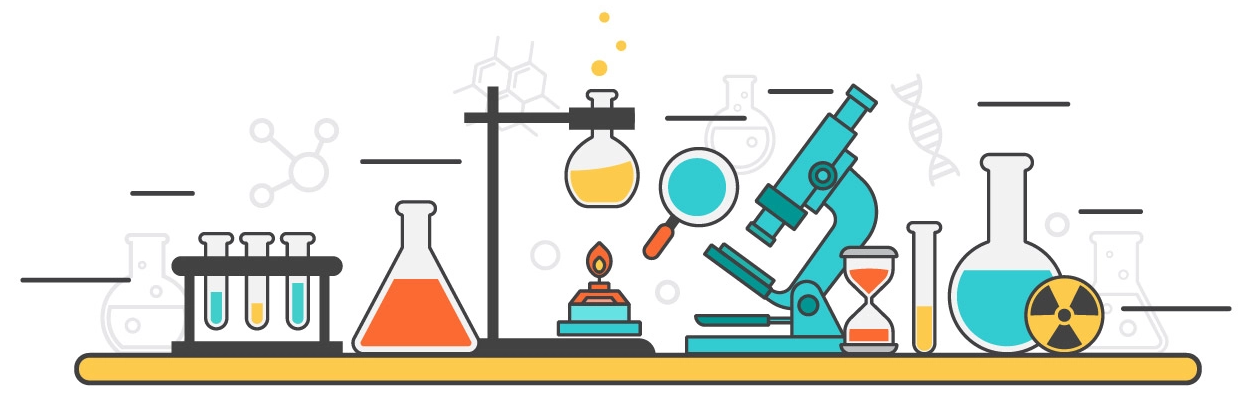
\includegraphics[width=\paperwidth]{../Unidad 2/Images/cover_bg}
\end{document}

\restoregeometry
\addtocontents{toc}{\setcounter{tocdepth}{3}}
\tableofcontents
\newpage
\chapter{}
\pagestyle{fancy}
\newpage \thispagestyle{plain}
\section{Nuestro mundo químico}
\subsection{La química en tu vida y el medio ambiente }

\newpage \thispagestyle{plain}
\section{Los materiales, las sustancias y sus propiedades}
This is a sample of a section
\subsection{¿Cómo sabemos que un material es distinto de otro?}
\subsection{¿Cómo podemos medir las propiedades de los materiales?}
\newpage \thispagestyle{plain}
\section{Relación entre propiedades de las sustancias e intercambios de energía}
\subsection{¿Cómo utilizamos energía para analizar sustancias?}

\newpage \thispagestyle{plain}
\section{Mezclas: propiedades y métodos de separación}

\subsection{Propiedades y clasificación de las mezclas}

\newpage \thispagestyle{plain}
\section{Mezclas y sustancias contaminantes}
\subsection{¿Cómo detectamos y prevenimos la presencia de sustancias nocivas en el medio ambiente?}

\subsection{Métodos de separación de mezclas}

\newpage \thispagestyle{plain}
\section{Sustancias elementales y sus propiedades}
\subsection{¿Hay sustancias más simples que otras?}
\subsection{Regularidades en las propiedades de las sustancias elementales}

\newpage
\chapter{}
% \begin{minipage}{.45\textwidth}
%   \begin{figure}[H]
%     \centering
%     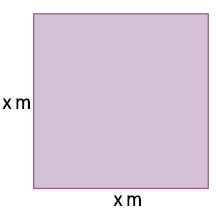
\includegraphics[width=0.7\linewidth]{square.png}
%     \captionof{figure}{Modelo geométrico de la situación.}
%     \label{fig:square}
%   \end{figure}%
% \end{minipage}\hfill
% \begin{minipage}{.45\textwidth}
%   \begin{figure}[H]
%     \centering
%     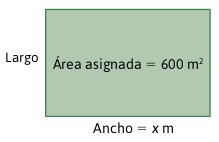
\includegraphics[width=0.8\linewidth]{square2.png}
%     \captionof{figure}{Modelo geométrico de la situación.}
%     \label{fig:square2}
%   \end{figure}
% \end{minipage}
\newpage \thispagestyle{plain}
\section{La estructura de la materia y sus modelos}
\boxabstract{
  \begin{itemize}
    \item Deduce información acerca de la estructura atómica
          a partir de datos experimentales sobre propiedades
          atómicas periódicas.
    \item Representa y diferencia mediante esquemas, modelos y
          simbología química, elementos y compuestos, así como
          átomos y moléculas.
    \item Explica y predice propiedades físicas de los materiales
          con base en modelos submicroscópicos sobre la
          estructura de átomos, moléculas o iones, y sus
          interacciones electrostáticas.
  \end{itemize}
}
%\newpage
\subsection{¿Cómo los átomos y las moléculas hacen distintas a las sustancias?}

\begin{boxK}
  \begin{enumerate}
    \item Anota en la tabla dos propiedades que distinguen a las sustancias que se indican y con
          las que de seguro estás en contacto frecuentemente.
    \item Dibuja qué verías si observaras cada sustancia con un microscopio muy potente.
    \item Compara tus ideas y dibujos con los de un compañero y comenten: \\
          \textbf{¿cómo explican sus dibujos las propiedades macroscópicas de las sustancias que representaron?}
          \begin{figure}[H]
            \centering
            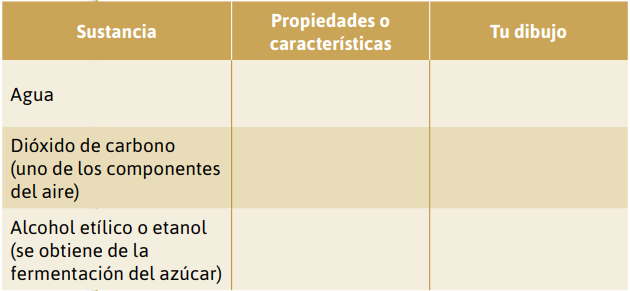
\includegraphics[width=0.7\linewidth]{tabla01.png}
            %\captionof{table}{Modelo geométrico de la situación.}
            \label{tab:tabla01}
          \end{figure}%
  \end{enumerate}
\end{boxK}

\subsubsection{\'Atomos y moléculas}

¿Por qué el carbón es una sustancia sólida negra y quebradiza que se quema con facilidad?
¿Por qué el azúcar es dulce y se disuelve en el agua? A lo largo de la historia, los químicos han realizado
diversos experimentos para comprender por qué cada sustancia tiene propiedades distintas.\\

Los resultados experimentales se pueden explicar mediante el modelo
cinético de partículas que estudiaste en tu curso de Ciencia y tecnología, Física, el cual supone que:

\begin{figure}[H]
  \centering
  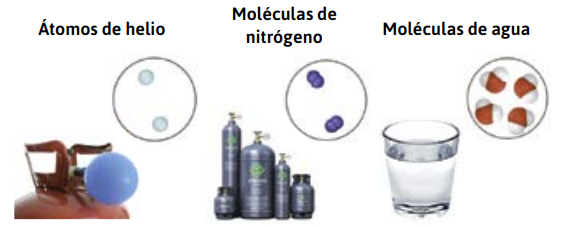
\includegraphics[width=.6\linewidth]{atomos01.png}
  \captionof{figure}{\footnotesize Representación de las partículas que constituyen diversas
    sustancias. Los átomos de distintos tipos se representan comúnmente
    como esferas de diferente color.}
  \label{fig:atomos01}
\end{figure}

%\begin{boxM}
\begin{itemize}
  \item[\checkmark] Las sustancias están constituidas por miles de millones de partículas pequeñísimas
        en constante movimiento e interacción;
  \item[\checkmark] Las partículas de una sustancia son idénticas entre sí y tienen una composición y
        estructura determinadas, que son diferentes a las de otras sustancias;
  \item[\checkmark] Las partículas de cada sustancia por lo general están constituidas por unidades más
        pequeñas llamadas \textbf{átomos}, unidos unos a otros por fuerzas de atracción llamadas \textbf{enlaces químicos}.
\end{itemize}
%\end{boxM}

Algunas sustancias elementales, como el helio y el argón, están constituidas por partículas de un solo átomo; sin embargo, las
partículas de muchas otras sustancias se forman por la unión, mediante enlaces químicos, de dos o más átomos; a estas partículas
se les llama \textbf{moléculas} (figura \ref{fig:atomos01}).

Por ejemplo, el gas nitrógeno del aire está constituido por moléculas de dos átomos
idénticos, mientras que las moléculas de agua están formadas por dos átomos de
hidrógeno unidos a un átomo de oxígeno (átomos de diferente tipo).
Las diferencias en las propiedades de las sustancias se deben a los distintos tipos
y números de átomos de las partículas que las constituyen y a la forma en que los
átomos se enlazan unos a otros.\\

\begin{boxK}
  \begin{wrapfigure}{r}{0.25\textwidth}
    \centering
    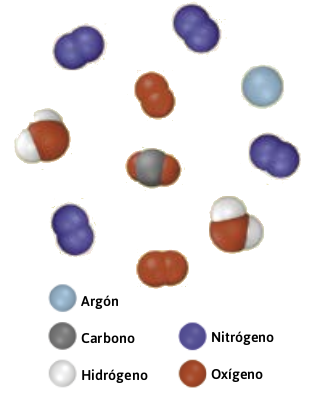
\includegraphics[width=0.25\textwidth]{atomos02.png}
    \label{fig:atomos02}
  \end{wrapfigure}
  Analiza y reflexiona:\\
  \begin{enumerate}
    \item Observa la representación de las partículas que
          forman algunas sustancias del aire que respiras.
          El código de color que por lo común se utiliza
          para representar átomos de distintos tipos es el
          que se muestra.
    \item Determina cuántas sustancias distintas se representan.
    \item Determina qué sustancias están constituidas por átomos independientes y cuáles por moléculas.
    \item Describe las semejanzas y diferencias de las moléculas que identificaste: considera tipo y cantidad de átomos.
    \item Compara tus respuestas con las de tus compañeros y valídenlas.
  \end{enumerate}%
  % \end{minipage}
\end{boxK}

\subsubsection{Sustancias elementales y compuestos químicos a nivel nanoscópico}

Como estudiaste en la unidad anterior, existen sustancias elementales que no se pueden descomponer
en otras más simples mediante procesos químicos. El nitrógeno y el oxígeno del aire son
ejemplos de sustancias elementales. Por otro lado, los compuestos
químicos sí se descomponen en sustancias elementales a partir
de métodos químicos. Algunos ejemplos son el agua, que puede
descomponerse en hidrógeno y oxígeno, y el dióxido de carbono
que exhalamos, que se descompone en oxígeno y carbono.\\

\begin{wrapfigure}{r}{0.4\textwidth}
  \centering
  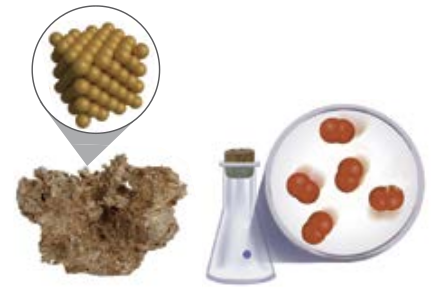
\includegraphics[width=0.4\textwidth]{atomos03.png}
  \captionof{figure}{\footnotesize El cobre y el oxígeno son sustancias
    elementales constituidas por átomos del mismo
    tipo.}
  \label{fig:atomos03}
\end{wrapfigure}

La idea de que las sustancias están constituidas por diferentes
tipos de átomos permite explicar la diferencia entre sustancias elementales y
compuestos químicos. Las elementales no pueden descomponerse en sustancias más simples porque están constituidas
por partículas con el mismo tipo de átomo.\\

\begin{wrapfigure}{l}{0.4\textwidth}
  \centering
  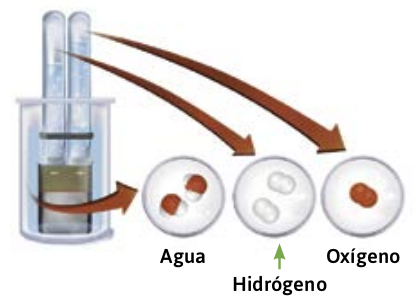
\includegraphics[width=0.4\textwidth]{atomos04.png}
  \captionof{figure}{\footnotesize El agua se logra descomponer en
    hidrógeno y oxígeno mediante el paso de
    corriente eléctrica.}
  \label{fig:atomos04}
\end{wrapfigure}

Por ejemplo, el cobre
con el que se fabrican cables, está conformado por átomos idénticos ordenados uno junto a otro,
mientras que el oxígeno que respiramos tiene moléculas con dos átomos de oxígeno cada una (figura
\ref{fig:atomos03}). Por su parte, los compuestos químicos se pueden descomponer en sustancias elementales
porque están constituidos por partículas
con átomos de distintos tipos. Los átomos que conforman las moléculas de agua, por ejemplo, se pueden separar
y reorganizarse para
formar las sustancias elementales hidrógeno y oxígeno (figura \ref{fig:atomos04}).\\

\subsubsection{Tipos de \'atomos}

La separación e identificación de las diferentes sustancias elementales que
hay en la naturaleza ha permitido determinar los distintos tipos de átomos
que existen. En la actualidad se han identificado más de 100 átomos
distintos, y las partículas de todas las sustancias conocidas, naturales o sintéticas,
son resultado de la combinación de esos átomos
(figura \ref{fig:atomos07}). Cada tipo de átomo corresponde con un elemento
químico y se le asigna un símbolo particular.

Por ejemplo, los
átomos de oxígeno se representan con el símbolo \emph{O}, mientras que
los átomos de hidrógeno, con el símbolo \emph{H}. Los símbolos que representan
cada tipo de átomo no siempre corresponden con las primeras letras
de su nombre en español, porque algunos se derivan del nombre de las sustancias
en otros idiomas, como el latín.\\

\begin{minipage}{\textwidth}
  \begin{boxK}
    Observa y representa:

    \begin{enumerate}
      \item Distingue similitudes y diferencias en las representaciones de las siguientes
            moléculas de distintas sustancias.

            \begin{figure}[H]
              \centering
              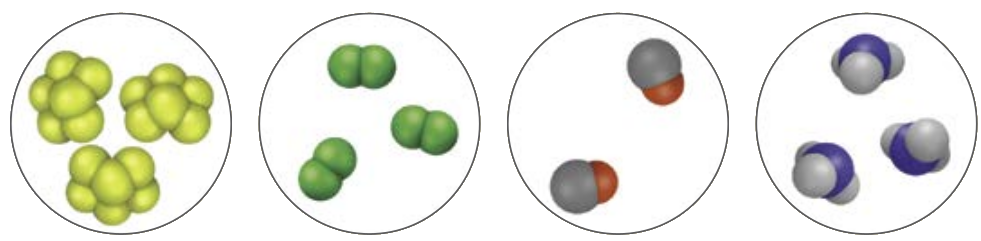
\includegraphics[width=.6\textwidth]{atomos05.png}
            \end{figure}

      \item Identifica cuáles representan sustancias elementales y cuáles compuestos quí-
            micos. Justifica tus decisiones.
      \item Usa las representaciones anteriores para representar una mezcla constituida por
            partículas de una sustancia elemental y partículas de un compuesto químico.
      \item Compara y contrasta tus dibujos con los de tus compañeros.
    \end{enumerate}
  \end{boxK}
\end{minipage}
\vspace{0.5cm}

\begin{wrapfigure}{l}{0.4\textwidth}
  \centering
  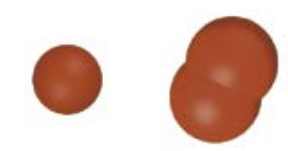
\includegraphics[width=0.3\textwidth]{atomos07.png}
  \captionof{figure}{\footnotesize Las propiedades y estructura de estas sustancias son diferentes aunque tengan el mismo tipo de átomo.}
  \label{fig:atomos07}
\end{wrapfigure}

Para el sodio, por ejemplo, el símbolo es Na porque proviene de su nombre en latín, natrium, que significa raro.
Los diferentes átomos o elementos químicos conocidos se listan en la
tabla periódica de los elementos (figura \ref{tab:periodic_table}, p. \pageref{tab:periodic_table}). Los que se localizan en la misma hilera pertenecen
al mismo periodo. Los átomos o elementos incluidos en la tabla periódica tienen el mismo
nombre que la sustancia elemental en la que están presentes, pero las propiedades de esos átomos no son
las mismas que las de las sustancias elementales.\\

\begin{wrapfigure}{l}{0.45\textwidth}
  \centering
  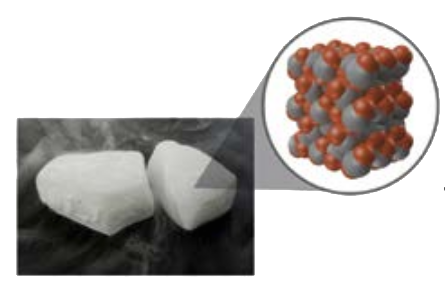
\includegraphics[width=0.45\textwidth]{atomos06.png}
  \captionof{figure}{\footnotesize El hielo seco (dióxido de
    carbono sólido) es un compuesto químico constituido por los elementos carbono y oxígeno.}
  \label{fig:atomos06}
\end{wrapfigure}

Por ejemplo, el oxígeno gaseoso presente en el aire que respiramos
está constituido por moléculas de dos átomos de oxígeno cada una. Los seres
humanos inhalamos sin problema las moléculas de oxígeno contenidas en
el aire, pero si en lugar de moléculas respiráramos átomos de oxígeno sepa-
rados, podríamos morir (figura \ref{fig:atomos06}).\\

Las propiedades de las sustancias elementales no sólo dependen del tipo de átomos que las componen, sino también
de cómo estos se enlazan en las partículas que los constituyen.
Por ejemplo, el grafito que contiene la punta de los lápices
es una sustancia elemental suave y quebradiza hecha de
átomos de carbono (C), mientras que el diamante, que es duro
y resistente, también es una sustancia elemental formada por
átomos de carbono (figura \ref{fig:atomos07}).\\

\begin{boxK}
  Analiza y genera hipótesis
  \begin{enumerate}
    \item Discute con tus compañeros sobre cómo es posible que
          dos sustancias con propiedades tan distintas como el
          diamante y el grafito estén constituidas por el mismo
          tipo de átomos (carbono, C).
  \end{enumerate}
\end{boxK}

\subsubsection{Simbología química}

Los químicos han desarrollado distintas maneras de representar la composición y
estructura de las sustancias elementales y de los compuestos químicos de nuestro
entorno (nivel macroscópico) mediante dibujos que representan los átomos y moléculas presentes en el material.
Cuando describimos el comportamiento de las sustancias
y los materiales representando los átomos y moléculas que los forman se dice que
hacemos una descripción a nivel nanoscópico.
En estas representaciones usamos fórmulas químicas que se hacen a partir de los
símbolos de los átomos o elementos químicos. Si las moléculas poseen átomos iguales,
se usan subíndices para indicar el número de átomos de cada tipo. Por ejemplo, la
fórmula química de las moléculas del oxígeno que respiramos es O$_2$ , lo cual indica que
cada una está constituida por dos átomos de oxígeno. La fórmula química de las moléculas de dióxido de carbono es CO$_2$;
esto indica que están formadas por un átomo de
carbono y dos de oxígeno. Si se necesita representar una sustancia con gran cantidad
de partículas en estado sólido, líquido o gaseoso, los símbolos (s), (l) y (g) se colocan a
la derecha de la fórmula: CO$_2$ (s) representa una muestra de dióxido de carbono sólido
(hielo seco) y O$_2$ (g) representa una muestra de oxígeno gaseoso.\\

En esta lección has aprendido que las diferencias en las propiedades de las sustancias
se deben a la composición de las partículas que las constituyen, la cual se representa
mediante esquemas que muestran la composición atómica de las partículas o el uso
de fórmulas químicas. Para evaluar lo que has aprendido, haz la siguiente actividad.

\newpage
\begin{landscape}
  \thispagestyle{plain}
  %\newgeometry{left=-50mm,top=-30mm,bottom=-30mm,right=-30mm}
  \begin{figure}[H]
    \TablaPeriodica[0.48]
    \captionof{table}{Tabla Peri\'odica de los Elementos.}
    \label{tab:periodic_table}
  \end{figure}
  %\restoregeometry
\end{landscape}

\newpage
\begin{boxK}
  \begin{enumerate}
    \item Completa la información de la tabla.
    \item Compara y contrasta la composición de las partículas que constituyen las distintas sustancias.
    \item Compara estas representaciones con las que hiciste al inicio de esta lección
          (p. 100): ¿cómo cambiaron? ¿Qué ventajas y desventajas tiene una representación respecto a la otra?
          \begin{figure}[H]
            \centering
            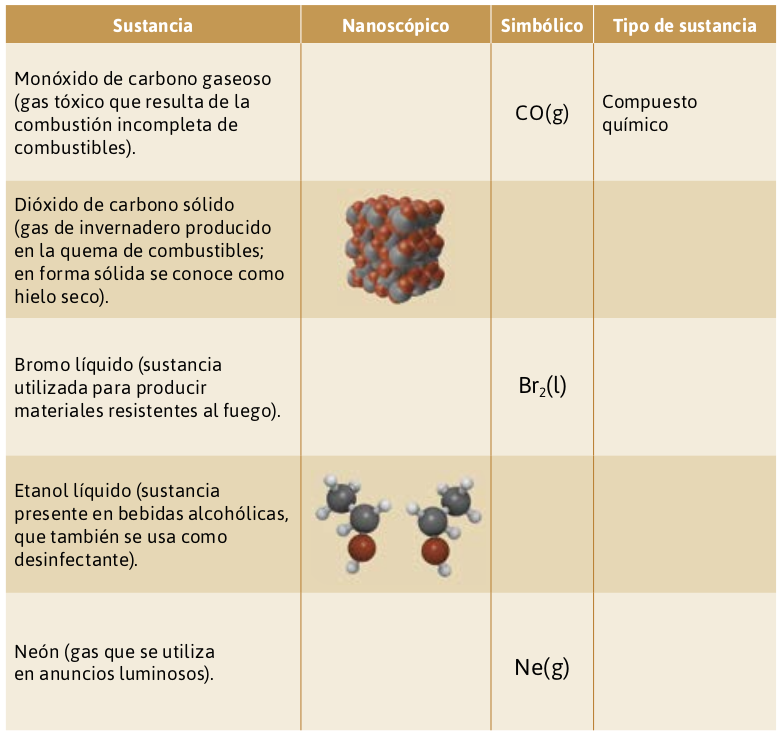
\includegraphics[width=.8\textwidth]{tabla02.png}
          \end{figure}

  \end{enumerate}
\end{boxK}

\newpage
\subsection{¿Qué hace a un átomo diferente de otro?}

\begin{boxK}
  \begin{enumerate}
    \item Explora las propiedades eléctricas de distintos materiales; por ejemplo, infla un globo
          (también puedes utilizar un vaso de plástico) y frótalo sobre tu cabello. Enseguida,
          acerca el globo a distintos materiales, como pequeños trozos de papel,
          una bolsa de plástico, un vaso de unicel, una lata de aluminio o un
          chorro fino de agua y de otras sustancias.
    \item Observa qué pasa en cada caso.
    \item Discute con tus compañeros por qué piensas que el material del que
          está hecho el globo interacciona de diferentes maneras con los otros
          materiales. Recuerda lo que aprendiste en tu curso de Ciencia y tecnología,
          Física sobre interacciones eléctricas.
    \item Discutan qué sucede a nivel nanoscópico con los átomos y las moléculas
          de las que están hechos estos materiales cuando los frotan.
  \end{enumerate}

\end{boxK}

\subsubsection{Componentes atómicos}

Un gran número de experimentos, como el propuesto en la actividad de inicio, sugieren
que la materia tiene propiedades eléctricas. En tu curso de Física aprendiste que
científicos como Thomson y Rutherford, a partir de distintos experimentos, detectaron
partículas (llamadas subatómicas) con cargas positivas y negativas en los átomos
y moléculas que constituyen las sustancias químicas. Con esta información propusieron
modelos para describir la estructura de los átomos, como el que se representa en
la figura \ref{fig:atomos08}.\\

\begin{figure}[H]
  \centering
  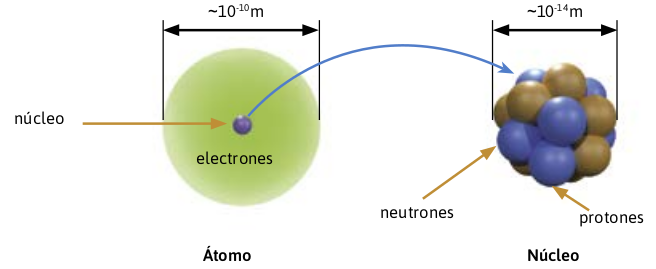
\includegraphics[width=0.7\linewidth]{atomos08.png}
  \captionof{figure}{\footnotesize Representación de la estructura de un átomo.}
  \label{fig:atomos08}
\end{figure}%

De acuerdo con este modelo atómico, cada átomo está constituido por partículas
con carga positiva, llamadas \textbf{protones}, concentradas en un núcleo muy pequeño, y por
partículas con carga negativa, denominadas \textbf{electrones}, que se mueven a su alrededor.
El núcleo de los átomos contiene otro tipo de partículas sin carga eléctrica (partículas
neutras) conocidas como \textbf{neutrones}. Los electrones son partículas muy pequeñas y
ligeras (poca masa), mientras que los protones y neutrones son de mayor tamaño y
poseen una masa 2 000 veces mayor que la del electrón. Cada átomo tiene el mismo
número de protones que de electrones y, por tanto, es eléctricamente neutro. Los electrones
se mantienen en movimiento alrededor del núcleo por la atracción entre cargas
eléctricas negativas y positivas.


\begin{boxK}
  Compara y analiza:\\
  \begin{enumerate}
    \item Lee y usa la información que se muestra en la imagen para determinar cuántas
          veces es más pequeño un átomo comparado con los objetos y organismos. Si es
          necesario, investiga el valor de las unidades de medida representadas.
          \begin{boxF}
            Los átomos son partículas muy pequeñas. En el diámetro de uno de tus cabellos se podrían
            acomodar en hilera unos 500 000 átomos de carbono. Si un cabello se pudiera agrandar
            hasta alcanzar el diámetro de nuestro planeta, un átomo del cabello tendría el tamaño de
            una cancha de basquetbol.
          \end{boxF}

          \begin{figure}[H]
            \centering
            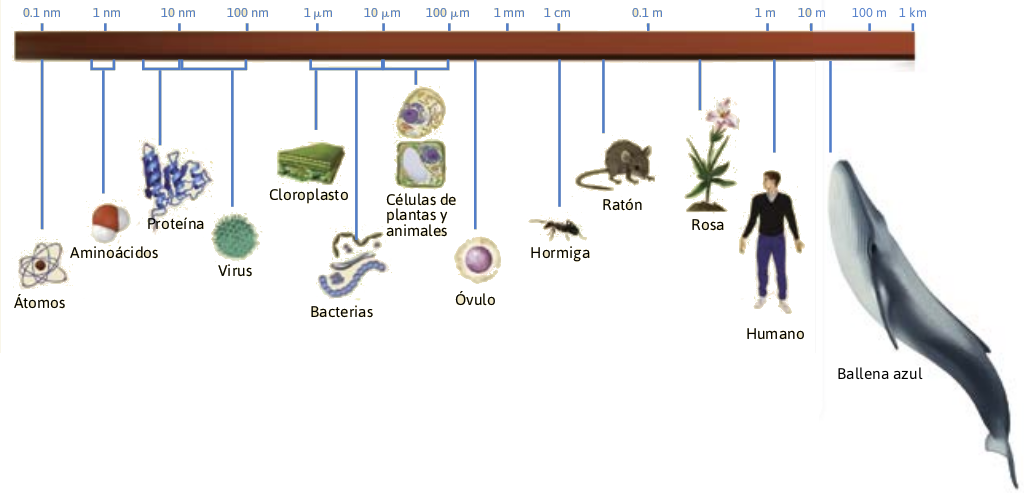
\includegraphics[width=.8\textwidth]{escala.png}
          \end{figure}


    \item Compara tus respuestas y métodos con los de otros compañeros y valídenlos.
  \end{enumerate}
\end{boxK}
\newpage

\subsubsection{Identidad atómica}

\begin{wrapfigure}{r}{0.35\textwidth}
  \centering
  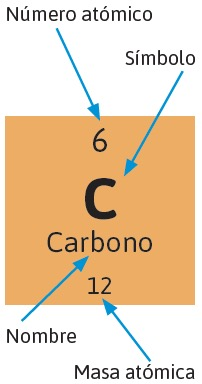
\includegraphics[width=0.45\linewidth]{eolementoCarbono.jpg}
  \captionof{figure}{\footnotesize Es importante reconocer cómo se presenta en la tabla periódica la información de cada átomo.}
  \label{fig:eolementoCarbono}
\end{wrapfigure}%

La identidad de cada átomo la determina su número de protones. Este dato se conoce como \textbf{número atómico} y
se representa con la letra Z. Por ejemplo, el átomo de hidrógeno (H) tiene en su núcleo un solo protón;
por tanto, su número atómico es Z = 1; el átomo de carbono (C) tiene seis protones y su número atómico
Z = 6. Como cada átomo es neutro, posee el mismo número de protones que de electrones; entonces, el número
atómico también indica cuántos electrones hay en cada átomo; así, el oxígeno (O) con Z = 8 está constituido
por 8 protones en el núcleo y 8 electrones que se mueven a su alrededor. El número atómico, Z, es la propiedad
que permite ordenar a los átomos de manera secuencial en la tabla periódica, y su valor se coloca sobre el símbolo
de cada elemento, como se ve en la figura \ref{fig:eolementoCarbono}.\\

La tabla periódica también contiene información sobre la \textbf{masa atómica relativa} de los distintos átomos y se
simboliza por las letras A$_r$ (figura \ref{fig:eolementoCarbono}). Medir la masa de un solo átomo es muy difícil,
pero es posible determinar cuántas veces la masa de un átomo es más grande en relación con otro.
Por ejemplo, de acuerdo con la tabla periódica,
A$_r$ = 12.0 para los átomos de carbono y Ar = 1.01 para los de hidrógeno. Esto indica que un solo átomo de carbono
es casi doce veces más pesado que uno de hidrógeno. Por su parte, la masa atómica relativa del magnesio (Mg)
es $A_r = 24.3$, lo cual implica que un átomo de este elemento es alrededor de 24 veces más pesado que uno de
hidrógeno, pero sólo dos veces más pesado que uno de carbono ($24.3/12 \sim 2$).\\

\begin{minipage}{\textwidth}
  \begin{boxK}
    Analiza e infiere:
    \begin{enumerate}
      \item Lee y organiza con tus compañeros un juego con base en preguntas y respuestas sobre cómo un átomo se compara
            con otros de la tabla periódica. Utiliza los ejemplos que se presentan más abajo como guía para proponer tus preguntas.

            \begin{boxF}
              Es importante que te familiarices con las propiedades de los átomos que forman las sustancias de tu alrededor,
              como el agua (H$_2$O), el azúcar (C$_{12}$H$_{22}$O$_{11}$) y el cloruro de sodio (sal común, NaCl).
              Estos átomos suelen tener números atómicos menores a 30 (Z < 30) y se localizan en las cuatro primeras hileras de
              la tabla periódica.
            \end{boxF}
      \item ¿Cuántas veces es más pesado un átomo de calcio (Ca) que un átomo de oxígeno (O)?
      \item ¿Cuántos electrones hay en un átomo de hierro (Fe)?
      \item ¿Cuántos protones más tiene un átomo de cloro que uno de carbono (C)?
    \end{enumerate}
  \end{boxK}
\end{minipage}

\newpage
\subsubsection{Ejercicios}

\begin{boxK}
  Elige la(s) respuesta(s) correcta(s).
  \begin{enumerate}
    \item ¿Qué propiedad periódica de los elementos se representa con la letra $Z$?

          \begin{hoptboxes}
            \item Densidad atómica
            \item Tamaño atómico
            \item Masa atómica
            \item Número atómico
          \end{hoptboxes}

    \item ¿A qué cantidad de partículas equivale $Z$?

          \begin{hoptboxes}
            \item Al número de neutrones.
            \item Al número de fotones.\\
            \item Al número de electrones.
            \item Al número de protones.
          \end{hoptboxes}
    \item ¿Qué propiedad periódica de los elementos se representa como $A_r$?

          \begin{hoptboxes}
            \item Densidad atómica relativa.
            \item Tamaño atómico relativo.\\
            \item Masa atómica relativa.
            \item Número atómico relativo.
          \end{hoptboxes}
    \item El valor $A_r=5$ para los átomos de boro significa que:

          \begin{hoptboxes}
            \item un sólo átomo de boro es casi 5 veces más pesado que uno de hidrógeno.\\
            \item un sólo átomo de hidrógeno es casi 5 veces más pesado que uno de boro.\\
            \item un sólo átomo de boro es casi 5 veces menos pesado que uno de hidrógeno.\\
            \item un sólo átomo de hidrógeno es casi 5 veces menos pesado que uno de boro.
          \end{hoptboxes}
    \item ¿Qué valor de $Z$ tiene un átomo con 20 neutrones y un valor de $A_r=39$?

          \begin{hoptboxes}
            \item Z = 20
            \item Z = 19
            \item Z = 49
            \item Z = 39
          \end{hoptboxes}

  \end{enumerate}

\end{boxK}

\subsubsection{Iones: partículas con carga eléctrica}

\begin{figure}[H]
  \centering
  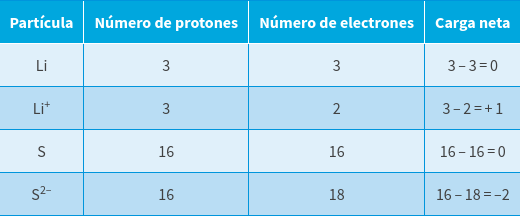
\includegraphics[width=0.7\linewidth]{tabla_de_cargas.png}
  \captionof{table}{Carga neta de algunos átomos.}
  \label{tab:tabla_de_cargas}
\end{figure}%

Los electrones de un átomo están en constante movimiento alrededor del núcleo atraídos por la carga positiva
de los protones. Como los electrones tienen carga negativa se repelen entre sí, lo que causa que algunos se
muevan cerca del núcleo atómico, mientras otros se desplazan a distancias más lejanas. Los electrones que están
más alejados del núcleo en ocasiones escapan del átomo o son atraídos por otros átomos o moléculas. Cuando esto
sucede, el átomo deja de tener el mismo número de protones y electrones y adquiere una carga eléctrica neta.
Se dice que se convierte en un \textbf{ion}.

\begin{figure}[H]
  \centering
  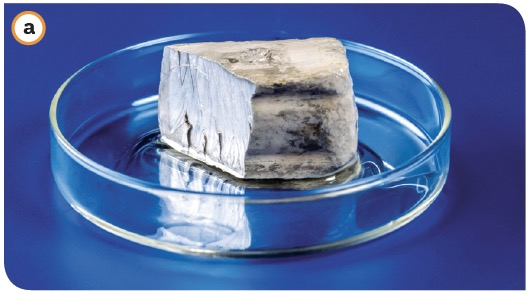
\includegraphics[width=0.40\linewidth]{sodio.jpg}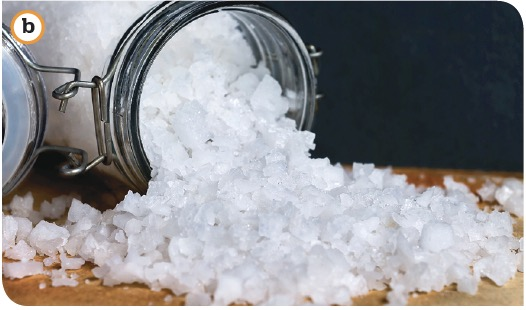
\includegraphics[width=0.40\linewidth]{sodio2.jpg}
  \captionof{figure}{\footnotesize El sodio metálico tiene propiedades muy diferentes al sodio de la sal común.
    a) Sodio metálico. b) Sal común contiene cationes de sodio (Na$^+$) y aniones de cloro (Cl$^-$).}
  \label{fig:sodio2}
\end{figure}%

Imagina, por ejemplo, que un átomo de litio (Li) con tres protones (Z = 3) perdiera uno de sus electrones.
Esta partícula tendría tres cargas positivas (+3), pero sólo dos cargas negativas (-2).
Su carga neta sería $+3 - 2 = +1$. Cuando esto sucede se dice que se forma un \textbf{ion positivo o catión},
y en el caso del litio este ion se representa con el símbolo Li$^+$. Un átomo también puede ganar electrones
atrayéndolos de otros átomos y así se transforma en un \textbf{ion negativo o anión}. Por ejemplo, si un átomo de
azufre (Z = 16) gana dos electrones, tendrá 16 protones y 18 electrones y su carga neta será $+16 - 18 = -2$.
Este anión se representa con el símbolo S$^{2-}$. La pérdida o ganancia de electrones no cambia la identidad de un
átomo, pero le da propiedades distintas. Los átomos de sodio (Na) en un pedazo de este metal interaccionan de
manera muy distinta con otras partículas a como lo hacen los iones Na+ presentes en compuestos químicos como
la sal común (figura \ref{sodio2}).


Muchos de los elementos químicos necesarios para la vida están presentes en todo nuestro cuerpo en forma de
iones, ya sea en los huesos, en la sangre y en el citoplasma de nuestras células.

\begin{boxK}
  Infiere y compara
  \begin{enumerate}
    \item Lee y completa la tabla con la información que se presenta.
          \begin{boxF}
            Muchos compuestos químicos a nuestro alrededor están constituidos por átomos o moléculas con carga, es decir,
            por aniones y cationes. Un ejemplo típico es el cloruro de sodio, simbolizado como NaCl, que está conformado por
            cationes Na$^+$ y aniones Cl$^-$. En la siguiente tabla se listan otros compuestos \emph{iónicos} importantes.
          \end{boxF}

          \begin{figure}[H]
            \centering
            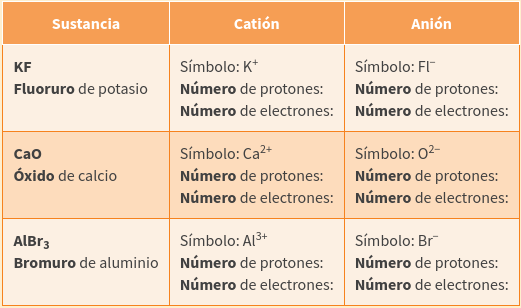
\includegraphics[width=0.6\linewidth]{tablaAnionCation.png}
            % \captionof{table}{El sodio metálico tiene propiedades muy diferentes al sodio de la sal común.
            %   a) Sodio metálico. b) Sal común contiene cationes de sodio (Na+) y aniones de cloro (Cl-).}
            \label{fig:tablaAnionCation}
          \end{figure}%

          Compara tus resultados con los de algunos compañeros de clase y valídenlos en grupo y con ayuda de su maestro.
          El modelo atómico de la materia es muy útil para explicar los fenómenos que observamos cada día; en particular, permite entender las interacciones entre diversas sustancias.
  \end{enumerate}
\end{boxK}
%
\begin{boxK}
  \begin{enumerate}
    \item Recuerda los experimentos que hiciste con el globo al principio de esta lección. Discute con tus compañeros qué sucede a nivel atómico cuando el globo se frota contra distintos materiales. Apliquen los conocimientos que adquirieron en esta lección sobre estructura atómica y formación de iones.
    \item Representen a nivel nanoscópico lo que le pasa a los electrones de los átomos en la superficie del globo y del cabello cuando se frotan el uno contra el otro. A partir de su representación expliquen lo siguiente.
          \begin{enumerate}
            \item Por qué el globo y el cabello se atraen después de frotarlos.
            \item Por qué el globo puede atraer otros materiales después de frotarlo.
          \end{enumerate}
    \item Compartan en equipos sus resultados, corríjanlos en caso de ser necesario y valídenlos con su maestro.
  \end{enumerate}
\end{boxK}

El modelo atómico de la materia es muy útil para explicar los fenómenos que observamos cada día;
en particular, permite entender las interacciones entre diversas sustancias.

\newpage
\subsection{¿Cómo estudiamos a los átomos de manera experimental?}
\begin{boxK}
  \begin{enumerate}
    \item Consigan en equipos cajas de cartón e introduzcan en ellas uno o varios objetos: lápices, gomas,
          llaves, etcétera; cada caja puede tener diferentes objetos. Cuiden que los otros equipos no vean
          lo que colocaron en las cajas.
    \item Séllenlas con cinta adhesiva de manera que no puedan ver su contenido.
    \item Intercambien su caja con otro equipo y sin abrirlas traten de descubrir qué objetos contienen.
    \item Después hagan lo que se indica.
          \begin{enumerate}
            \item Reflexionen en grupo sobre las pruebas o los experimentos que pueden realizar para determinar
                  el contenido de las cajas.
            \item Pongan a prueba sus ideas y traten de inferir el contenido de la caja.
          \end{enumerate}
    \item Comprueben sus respuestas abriendo las cajas. ¿Acertaron? ¿Se equivocaron? Expliquen.
  \end{enumerate}
\end{boxK}


\subsubsection{Descubriendo sin ver}

El problema al que te enfrentaste en la actividad anterior de tratar de saber qué hay en la caja sin verlo
es análogo al que se han enfrentado los científicos para descubrir la estructura de los átomos.
Para entender y explicar cómo los átomos se unen entre sí para formar las moléculas de los diferentes
tipos de sustancias se requiere explorar su estructura interna. Pero ¿cómo hacerlo si los átomos no se
pueden ver ni con el microscopio más potente? Es probable que al investigar el contenido de la caja en
la actividad inicial usaras diferentes formas de energía para determinar su contenido.
Por ejemplo, aplicaste energía mecánica para agitarla; aprovechaste la energía sonora para identificar
los sonidos de los objetos al chocar. De manera similar, los científicos se han valido de diversos desarrollos
tecnológicos que les permiten utilizar diferentes tipos de energía para explorar las propiedades de los átomos.

\begin{figure}[H]
  \centering
  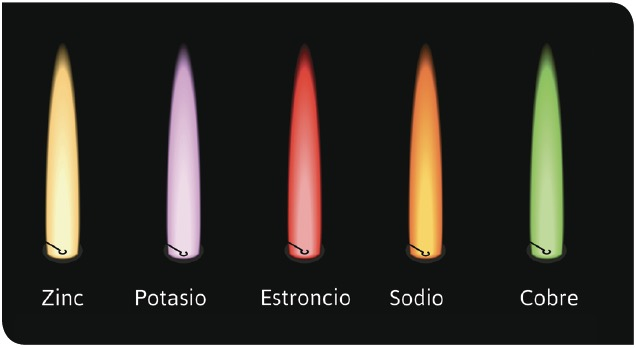
\includegraphics[width=0.5\linewidth]{flama.jpg}
  \captionof{figure}{\footnotesize Diferentes elementos químicos emiten luz de colores distintos.}
  \label{fig:flama}
\end{figure}%

Por ejemplo, en tu curso de Ciencia y tecnología, Física estudiaste que los científicos utilizaron energía
térmica para calentar muestras de diferentes elementos y analizar la luz que emitan (figura \ref{fig:flama}).
Este tipo de luz dio pistas sobre cómo se distribuyen y mueven los electrones alrededor del núcleo.



Los científicos también utilizan rayos X para medir el tamaño de los átomos.
La gráfica \ref{fig:radio_numero} muestra cómo el radio de los átomos cambia con el número atómico Z para los
primeros veinte elementos químicos de la tabla periódica.

\begin{figure}[H]
  \centering
  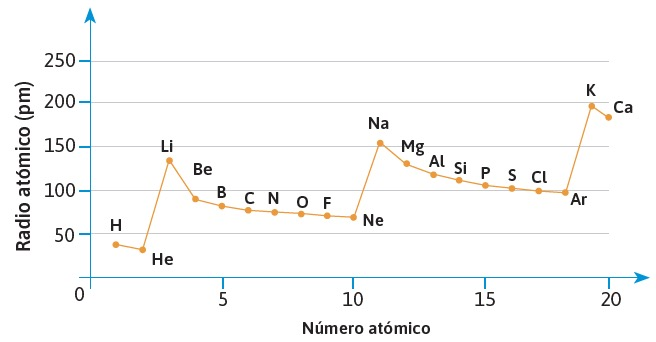
\includegraphics[width=0.8\linewidth]{radio_numero.jpg}
  \captionof{figure}{Variación del radio atómico (en picómetros) en función del número atómico
  }
  \label{fig:radio_numero}
\end{figure}%

\begin{boxF}
  Analiza e interpreta
  \begin{enumerate}
    \item Revisen en equipos los resultados experimentales que se presentan en la gráfica \ref{fig:radio_numero} sobre la variación del radio atómico en función del número atómico, Z, y respondan.
          \begin{enumerate}
            \item ¿Cómo cambia el radio de los átomos a medida que el número atómico se incrementa para elementos dentro de un mismo periodo (hilera) en la tabla periódica?
            \item ¿Y cómo varía a medida que el número atómico se incrementa para elementos dentro de un mismo grupo o familia (columna)?
            \item Utilicen los datos para justificar esta afirmación: el radio atómico es una propiedad \emph{periódica} de los elementos químicos.
            \item Propongan una hipótesis que explique las variaciones observadas en el radio de los átomos a medida que el número atómico de los elementos se incrementa en un mismo periodo y en una misma familia de la tabla periódica.
            \item Expongan ante el grupo sus hipótesis y validen sus argumentos.
          \end{enumerate}

  \end{enumerate}
\end{boxF}

\subsubsection{Modelo de capas}

Las investigaciones sobre la estructura de distintos tipos de átomos muestran que ciertas propiedades de estas partículas,
como el radio atómico, varían de manera periódica con el número atómico. ¿Cómo podemos explicar este comportamiento?
A lo largo de la historia se han propuesto diferentes modelos sobre la estructura de los átomos para explicar este fenómeno.
Uno de ellos se conoce como modelo de capas electrónicas, que es útil para entender la periodicidad atómica.


\begin{figure}[H]
  \centering
  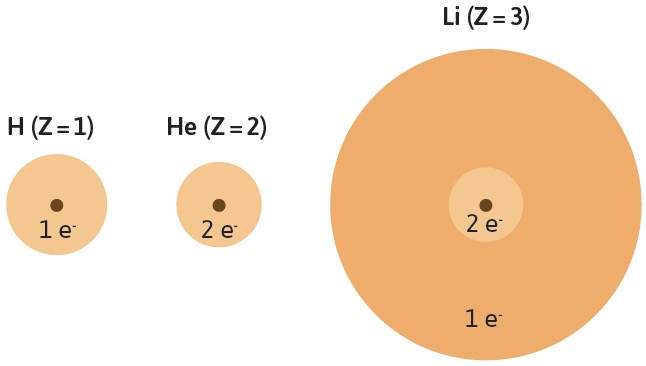
\includegraphics[width=0.4\linewidth]{capas01.jpg}
  \captionof{figure}{Distribución en capas de los electrones en los átomos de H, He y Li.}
  \label{fig:capas01}
\end{figure}

Los electrones de un átomo están en constante movimiento y no es posible determinar con precisión,
en un instante dado, su trayectoria y ubicación; sin embargo, sí se logra predecir la probabilidad de
encontrar electrones en diferentes regiones alrededor del núcleo. Para explicar los resultados
experimentales se ha propuesto que en un átomo los electrones tienden a localizarse en capas más o
menos esféricas alrededor del núcleo; sin embargo, como los electrones se repelen unos a otros, no
todos ellos están en la misma capa. Para ilustrar esta idea consideremos los tres primeros elementos
en la tabla periódica: hidrógeno (H, Z = 1), helio (He, Z = 2) y litio (Li, Z = 3).
La figura \ref{fig:capas01} ilustra cómo se distribuyen los electrones de esos átomos de acuerdo
con el modelo de capas electrónicas.



El electrón en el átomo de hidrógeno se mueve en la primera capa. En el átomo de helio, los dos electrones
también se desplazan dentro de la primera capa, pero como el átomo de helio tiene un protón más que el átomo
de hidrógeno, el núcleo atrae los dos electrones con más fuerza y por eso es un poco más pequeño que el átomo de hidrógeno.

El átomo de litio sólo tiene un electrón más que el átomo de helio, pero su tamaño es mucho mayor (figura \ref{fig:capas01}).
Para explicarlo suponemos que en el átomo de litio la repulsión entre electrones causa que el tercer electrón ocupe una capa
distinta, más alejada del núcleo. Varios electrones pueden moverse dentro de la misma capa atómica, pero hay un punto en
el que las repulsiones electrónicas obligan a los electrones adicionales a moverse en una capa más externa.
La figura \ref{fig:capas02} ilustra este fenómeno para los átomos del segundo periodo en la tabla periódica y
para el primer elemento del tercer periodo. En los átomos del segundo periodo, los dos primeros electrones se
localizan en la primera capa, y el resto se mueve en la segunda, la cual tiene la capacidad de alojar un máximo
de ocho electrones. Las interacciones entre éstos hacen que el electrón adicional en el átomo de sodio (Na, Z = 11)
se localice en una tercera capa, incrementando el tamaño de este átomo.

\begin{figure}[H]
  \centering
  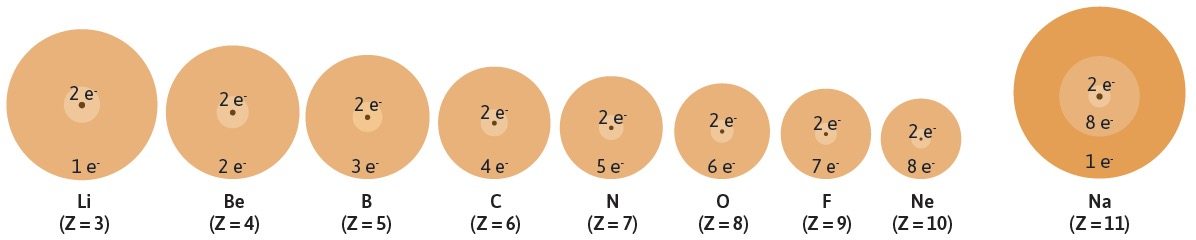
\includegraphics[width=0.9\linewidth]{capas02.jpg}
  \captionof{figure}{Distribución en capas de los electrones en átomos con Z = 3 hasta Z = 11.}
  \label{fig:capas02}
\end{figure}%

\begin{boxK}
  Analiza y explica
  \begin{enumerate}
    \item Lean y analicen en equipo cómo la energía de ionización cambia con el número atómico para elementos de un
          mismo periodo (hilera) de la tabla periódica y para elementos de un mismo grupo o familia (columna).

          \begin{boxF}
            La gráfica \ref{fig:radio_numero} muestra la energía necesaria para arrancar un electrón de la capa más
            externa de átomos
            con un número atómico entre Z=1 y Z=55. Esta energía se conoce como energía de ionización de los
            elementos, la cual entre más grande resulta más difícil para el átomo perder un electrón y convertirse en un catión.
          \end{boxF}

    \item Determina si la energía de ionización es una propiedad periódica. Justifiquen su respuesta.
    \item Expliquen, con base en el modelo atómico de capas, cómo varía la energía de ionización de los átomos a
          lo largo de un periodo y de una familia.
    \item Presenten sus respuestas y explicaciones al grupo y entre todos determinen si son lógicas y coherentes.
  \end{enumerate}
\end{boxK}
\newpage
\subsubsection{Ejercicios}
\begin{boxK}
  Relaciona la especie química con la cantidad de \textbf{protones} y \textbf{electrones de valencia}.\\

  \begin{minipage}{0.5\textwidth}
    \begin{enumerate}
      \item Magnesio (Mg)
      \item I\'on Potasio (K$^+$)
      \item Ión azufre (S2$^-$)
      \item Ión flúor (F$^-$)
      \item Ión calcio (Ca$_2^+$)
      \item Carbono (C)
      \item Ión aluminio (Al$_3^+$)
    \end{enumerate}
  \end{minipage}%
  % \vspace{2cm}
  \begin{minipage}{0.5\textwidth}
    \begin{itemize}
      \item[\rule{1cm}{0.2mm}] 20 protones y 8 electrones.
      \item[\rule{1cm}{0.2mm}] 9 protones y 8 electrones.
      \item[\rule{1cm}{0.2mm}] 16 protones y 8 electrones.
      \item[\rule{1cm}{0.2mm}] 6 protones y 4 electrones.
      \item[\rule{1cm}{0.2mm}] 13 protones y 8 electrones.
      \item[\rule{1cm}{0.2mm}] 19 protones y 8 electrones.
      \item[\rule{1cm}{0.2mm}] 12 protones y 2 electrones.
    \end{itemize}
  \end{minipage}

\end{boxK}

\begin{boxK}
  Relaciona la especie química con la cantidad de \textbf{protones} y \textbf{electrones de valencia}.\\

  \begin{minipage}{0.5\textwidth}
    \begin{enumerate}
      \item Ión oxígeno (O$_2^-$)
      \item Nitrógeno (N)
      \item Silicio (Si)
      \item Calcio (Ca)
      \item Neón (Ne)
      \item Ión Litio (Li$^+$)
      \item Fósforo (P)
      \item Selenio (Se)
    \end{enumerate}
  \end{minipage}%
  % \vspace{2cm}
  \begin{minipage}{0.5\textwidth}
    \begin{itemize}
      \item[\rule{1cm}{0.2mm}] 20 protones y 2 electrones.
      \item[\rule{1cm}{0.2mm}] 15 protones y 5 electrones.
      \item[\rule{1cm}{0.2mm}] 8 protones y 8 electrones.
      \item[\rule{1cm}{0.2mm}] 14 protones y 4 electrones.
      \item[\rule{1cm}{0.2mm}] 7 protones y 5 electrones.
      \item[\rule{1cm}{0.2mm}] 3 protones y 2 electrones.
      \item[\rule{1cm}{0.2mm}] 34 protones y 6 electrones.
      \item[\rule{1cm}{0.2mm}] 10 protones y 8 electrones.
    \end{itemize}
  \end{minipage}
\end{boxK}
\newpage
\begin{boxK}

  \begin{boxF}
    Aunque los átomos no se pueden observar ni con el microscopio más potente,
    a lo largo de la historia los científicos han propuesto distintos modelos
    de la estructura de estas partículas. Estos modelos se han construido y
    modificado con base en resultados de experimentos que, de manera indirecta,
    como cuando agitaste la caja cerrada en la actividad inicial, proporcionan
    información sobre su estructura atómica. Estos experimentos han sido posibles
    gracias al desarrollo de tecnologías que han permitido explorar de manera
    más precisa la estructura atómica.
  \end{boxF}
  \begin{enumerate}
    \item Analicen en equipos las principales características y limitaciones
          de los modelos atómicos propuestos por Dalton, Thomson, Rutherford y Bohr.
          Para ello revisen la infografía, y también consulten otros libros o sitios
          de internet confiables.
    \item Determinen qué desarrollos científicos y tecnológicos permitieron
          realizar los experimentos para obtener la información utilizada por Dalton,
          Thomson, Rutherford y Bohr en la elaboración de sus modelos atómicos.
    \item Elaboren con los resultados de su investigación una línea del tiempo que
          muestre la evolución histórica de los modelos atómicos y de los desarrollos
          científicos y tecnológicos que influyeron en su elaboración.
  \end{enumerate}
\end{boxK}
\newpage
\begin{landscape}
  \thispagestyle{plain}
  \begin{figure}[H]
    \centering
    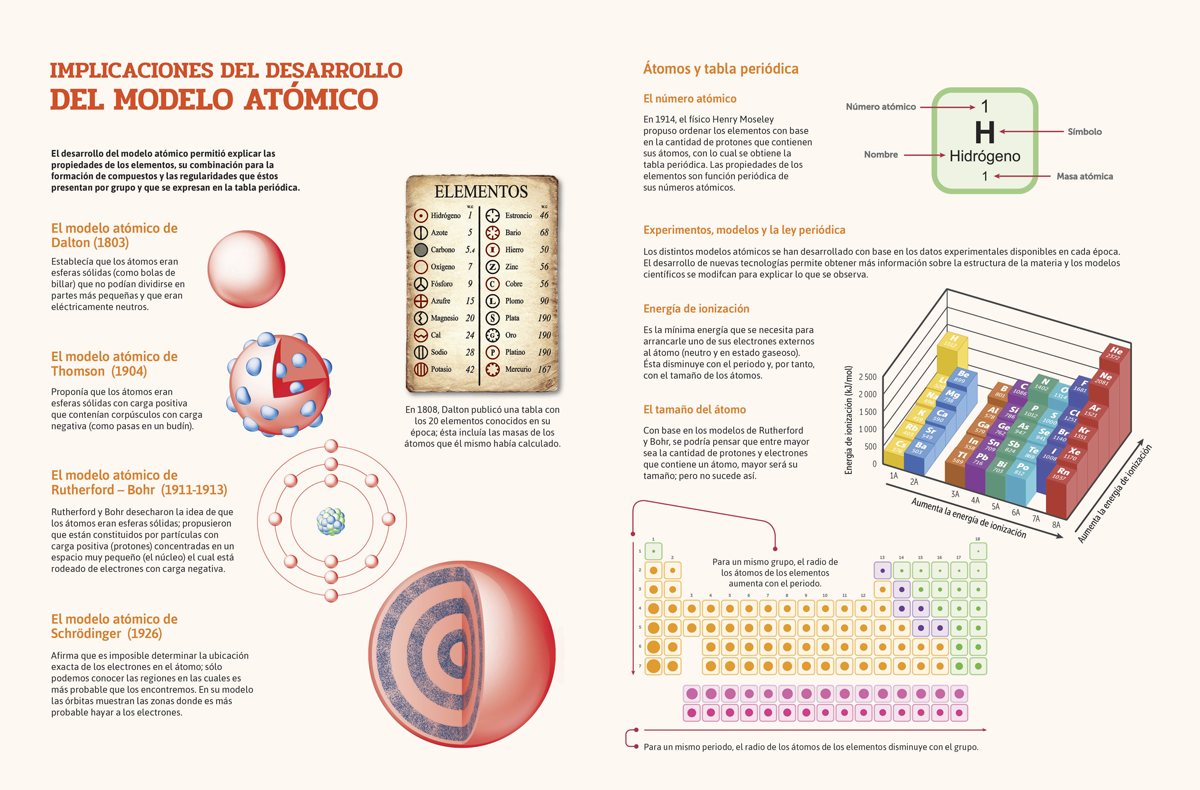
\includegraphics[width=\paperwidth]{SINQU3SB_1E16_U2_S7_114_115_INF.png}
    \label{fig:SINFI2SB_1E16_U1_S4_b_info}
    %\captionof{figure}{M\'aquinas simples.}
  \end{figure}
\end{landscape}

\newpage \thispagestyle{plain}
\section{Composición y estructura de distintos tipos de sustancias}

\boxabstract{
  \begin{itemize}
    \item Representa y diferencia mediante esquemas, modelos y
          simbología química, elementos y compuestos, así como
          átomos y moléculas.
    \item Explica y predice propiedades físicas de los materiales
          con base en modelos submicroscópicos sobre la
          estructura de átomos, moléculas o iones, y sus
          interacciones electrostáticas.
  \end{itemize}
}
%\newpage
\subsection{¿Qué tipos de partículas se forman al combinar los átomos?}
\begin{boxK}
  \begin{enumerate}
    \item La tabla \ref{tab:tabla_sustancias} presenta ejemplos de sustancias comunes. En la unidad 1 realizaste experimentos con algunas de ellas y estudiaste sus propiedades.
          \begin{figure}[H]
            \centering
            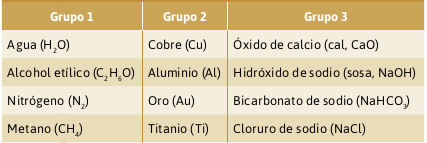
\includegraphics[width=.6\textwidth]{tabla_sustancias.png}
            \captionof{table}{Grupos de sustancias}
            \label{tab:tabla_sustancias}
          \end{figure}
    \item Describe propiedades comunes a las sustancias de cada grupo. Considera su apariencia física, estado de agregación, solubilidad en agua y conductividad eléctrica.
    \item Considera la composición y estructura de las partículas que componen las sustancias de cada grupo, y plantea hipótesis sobre qué genera esas propiedades.
    \item Comparte tus ideas con tus compañeros de grupo y reflexiona ¿coinciden las propiedades que observaste con las que ellos identificaron? Complementen sus descripciones.
  \end{enumerate}
\end{boxK}

\subsubsection{Los tipos de sustancias y sus diferencias}
Cada sustancia tiene propiedades diferentes, por ejemplo, algunas son solubles
en agua y otras no, o algunas conducen la electricidad mientras otras son aislantes
eléctricos. Existen diversas maneras de clasificar las sustancias con base en sus
propiedades, y una de ellas se muestra en la tabla \ref{tab:tabla_sustancias2}.

\begin{figure}[H]
  \centering
  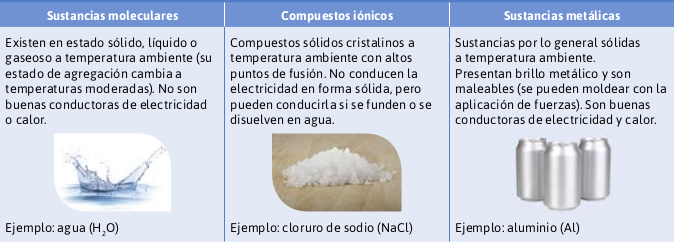
\includegraphics[width=\textwidth]{tabla_sustancias2.png}
  \captionof{table}{Tipos de sustancias y sus propiedades}
  \label{tab:tabla_sustancias2}
\end{figure}

\begin{boxK}
  Analiza y predice
  \begin{enumerate}
    \item Predice, con base en tus observaciones, experiencias y conocimientos adquiridos en este curso, a qué grupo
          (sustancias moleculares, compuestos iónicos o sustancias metálicas) pertenece cada uno de los siguientes materiales.
          Justifica tus predicciones de acuerdo con sus propiedades físicas.
          \begin{enumerate}
            \item Plata (Ag)
            \item Azúcar (C$_{12}$H$_{22}$O$_{11}$)
            \item Carbonato de calcio (CaCO$_3$)
            \item Acetona (C$_3$H$_6$O)
            \item Nitrato de sodio (salitre, NaNO$_3$)
            \item Hierro (Fe)
          \end{enumerate}
    \item Argumenta tus predicciones con tus compañeros.
  \end{enumerate}
\end{boxK}

Para explicar las propiedades de las sustancias moleculares, iónicas y metálicas, los científicos han propuesto
que las partículas que las constituyen tienen composición y estructura características. La estructura se refiere
a la manera en que los átomos o iones se agrupan. A continuación se describirán y analizarán las diferencias a
nivel nanoscópico entre estos tres grandes grupos de sustancias.



\subsubsection{Sustancias moleculares}

\begin{figure}[H]
  \centering
  \captionof{figure}{\footnotesize Atracción y repulsión entre protones y electrones durante la formación de una molécula.}
  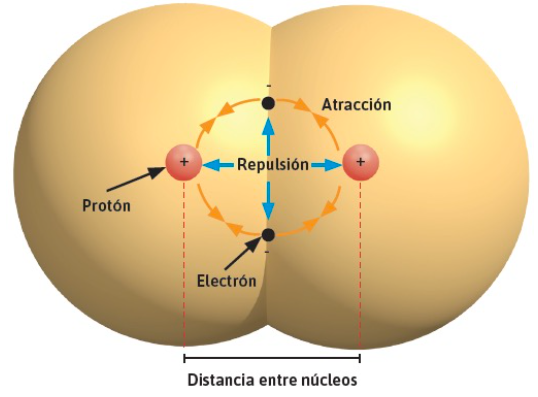
\includegraphics[width=.5\textwidth]{atraccion_repulsion.png}
  \label{fig:atraccion_repulsion}
\end{figure}

Para explicar que este tipo de sustancias no conduce la electricidad y tiene puntos de
ebullición y fusión relativamente bajos, se propuso que están constituidas por moléculas
neutras (su carga eléctrica neta es cero) que se forman cuando átomos del mismo o diferente
tipo se unen entre sí. Cada molécula se forma cuando dos o más átomos se acercan, y los
protones de uno atraen a los electrones de valencia del otro (figura \ref{tab:tabla_sustancias}). Esta fuerza
de atracción mantiene a los átomos juntos en la molécula.

Las \textbf{sustancias moleculares} son resultado de la combinación de elementos químicos conocidos
como \textbf{no metales}. Entre ellos se encuentran el hidrógeno y los elementos localizados en la
esquina superior derecha de la tabla periódica (figura \ref{tab:tabla_sustancias2}).
La unión entre dos átomos que forman una molécula por lo general se representa mediante
una línea, como se ilustra a continuación para la molécula de hidrógeno (H$_2$).

\begin{center}
  H - H
\end{center}

La línea entre los símbolos de los átomos representa la fuerza que los mantiene unidos.
A esta representación se le conoce como fórmula estructural, en este caso de la molécula
de hidrógeno, mientras que el símbolo H$_2$ se conoce como fórmula condensada.

\begin{figure}[H]
  \centering
  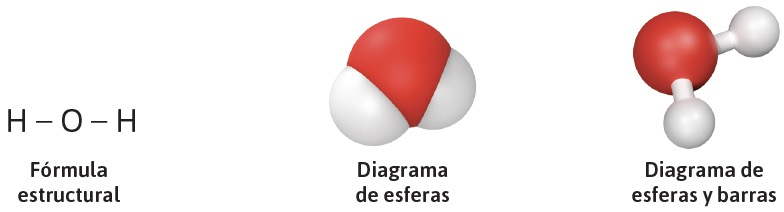
\includegraphics[width=0.8\textwidth]{esferas.jpg}
  \captionof{figure}{ Diferentes representaciones de la misma molécula. ¿Qué diferencias y semejanzas encuentras?}
  \label{fig:esferas}
\end{figure}

Algunos átomos de elementos no metálicos pueden unirse al mismo tiempo a más de un átomo.
Considera, por ejemplo, el caso de la molécula de agua: cada una tiene un átomo de oxígeno
unido a dos átomos de hidrógeno como se muestra en esta fórmula estructural:

\begin{center}
  H - O - H
\end{center}

Existen diversas formas de representar la unión de los átomos de las moléculas, y hoy en día,
con la ayuda de las computadoras, es posible generar imágenes tridimensionales de cualquier
molécula.

En la figura \ref{fig:esferas}, por ejemplo,
se ilustran algunas maneras de representar una molécula de agua (H$_2$O).

En los diagramas tridimensionales los átomos se representan como esferas. Los enlaces a
veces se muestran como barras que las conectan (diagramas de esferas y barras) o no se muestran de manera visible (diagramas de esferas).

Mediante el análisis de la composición química de múltiples sustancias moleculares,
se ha descubierto que cada tipo de átomo en general forma un número determinado de enlaces.
Por ejemplo, cada átomo de hidrógeno forma sólo un enlace con otros, mientras que cada
átomo de oxígeno forma dos enlaces.

El número de enlaces que cada tipo de átomo puede
formar se denomina capacidad de combinación del elemento o valencia. La figura \ref{fig:valencia}
muestra la valencia de los elementos no metálicos: la del hidrógeno es 1, lo cual
indica que este tipo de átomos sólo forma un enlace con otros; la del carbono es 4,
lo cual señala que este tipo de átomo típicamente forma cuatro enlaces con otros.

\begin{minipage}{.4\textwidth}
  \begin{figure}[H]
    \centering
    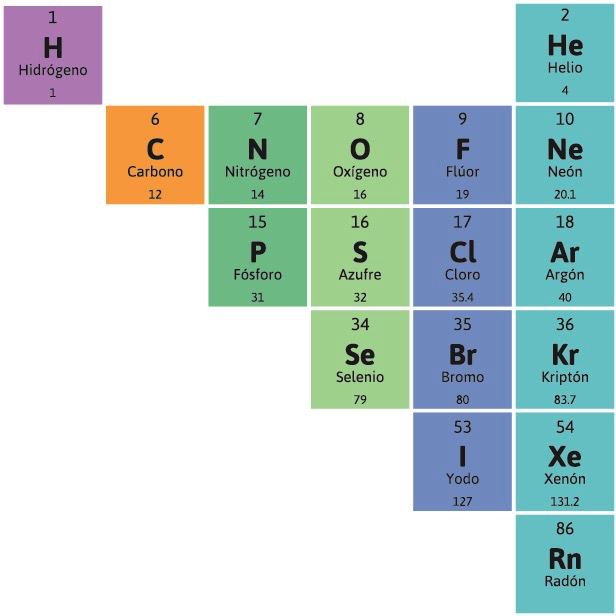
\includegraphics[width=0.5\textwidth]{no_metales.jpg}
    \label{fig:no_metales}
    \captionof{figure}{\footnotesize Elementos no metálicos.}
  \end{figure}
\end{minipage}\hfill
\begin{minipage}{.4\textwidth}
  \begin{figure}[H]
    \centering
    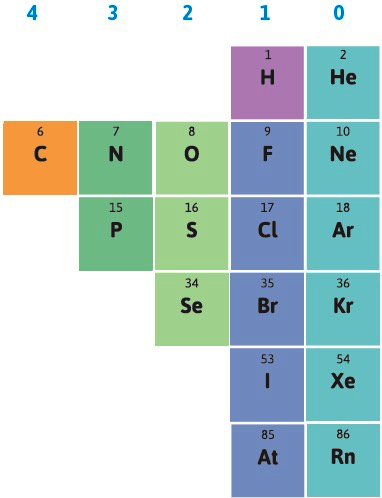
\includegraphics[width=0.5\textwidth]{valencia.jpg}
    \captionof{figure}{\footnotesize Valencia (capacidad de combinación) de diferentes tipos de átomos no metálicos.}
    \label{fig:valencia}
  \end{figure}
\end{minipage}

La valencia de los elementos es una propiedad periódica; esto significa que los átomos de elementos de un mismo grupo o familia (columna) de la tabla periódica en general forman el mismo número de enlaces cuando se combinan con otros. Este comportamiento facilita la predicción de la composición química y estructura de las moléculas que resultan al combinar distintos tipos de átomos de elementos no metálicos.

\begin{boxK}
  Representa e infiere
  \begin{enumerate}
    \item Considera la valencia o capacidad de combinación de los diferentes átomos no metálicos y representa la fórmula estructural de las moléculas que se forman cuando:
          \begin{enumerate}
            \item un átomo de carbono se combina con átomos de hidrógeno;
            \item un átomo de nitrógeno se combina con átomos de hidrógeno;
            \item un átomo de cloro se combina con átomos de hidrógeno.
          \end{enumerate}
    \item Escribe la fórmula condensada de las moléculas que se crean en cada caso. En esta fórmula primero se escribe el átomo que forma más enlaces.
    \item Compara y contrasta tus representaciones con las de algunos compañeros. Corríjanlas en caso de ser necesario.
  \end{enumerate}
\end{boxK}

En algunos casos, un átomo llega a formar más de un enlace con otro debido a que varios electrones de valencia de cada átomo son atraídos por los protones del otro. Por ejemplo, un átomo de carbono y uno de oxígeno pueden unirse con dos enlaces (enlace doble). En la molécula de dióxido de carbono, esto sucede como se ilustra a continuación.

\subsubsection{Ejercicios}
\begin{boxK}
  Relaciona la especie química con la cantidad de \textbf{protones} y \textbf{electrones de valencia}.\\

  \begin{minipage}{0.6\textwidth}
    \begin{enumerate}
      \item Las sustancias se representan con símbolos atómicos y líneas que simbolizan a los enlaces químicos.
      \item Esquema tridimensional en el que no es posible identificar a los enlaces químicos.
      \item Las sustancias se representan sólo con símbolos atómicos.
      \item Esquema tridimensional en el que es posible identificar a los enlaces químicos.
    \end{enumerate}
  \end{minipage}\hfill
  \begin{minipage}{0.3\textwidth}
    \begin{itemize}
      \item[\rule{1cm}{0.2mm}] Diagrama de esferas\\
      \item[\rule{1cm}{0.2mm}] Fórmula estructural\\
      \item[\rule{1cm}{0.2mm}] Fórmula condensada\\
      \item[\rule{1cm}{0.2mm}] Diagrama de esferas y barras\\
    \end{itemize}
  \end{minipage}

\end{boxK}

\begin{figure}[H]
  \centering
  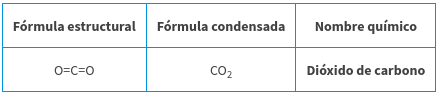
\includegraphics[width=0.6\textwidth]{formulas_co2.png}
  \label{fig:formulas_co2}
  % \captionof{figure}{  Valencia (capacidad de combinación) de diferentes tipos de átomos no metálicos.}
\end{figure}

Observa que en la fórmula estructural del dióxido de carbono el enlace doble se representa con dos líneas
paralelas entre los átomos. La fuerza de atracción entre los átomos unidos por un doble enlace es mayor
que la que existe entre aquellos unidos por un solo enlace.

\begin{figure}[H]
  \centering
  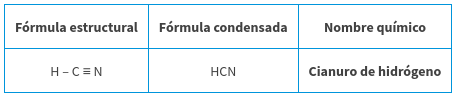
\includegraphics[width=0.6\textwidth]{formulas_hcn.png}
  \label{fig:formulas_hcn}
  % \captionof{figure}{  Valencia (capacidad de combinación) de diferentes tipos de átomos no metálicos.}
\end{figure}

Algunos átomos pueden formar entre ellos hasta tres enlaces (enlace triple),
como en la unión entre átomos de carbono y nitrógeno en el cianuro de hidrógeno,
un compuesto molecular muy tóxico. El enlace triple se representa con tres líneas
paralelas entre los átomos que se unen.

\begin{wrapfigure}{l}{0.4\textwidth}
  \centering
  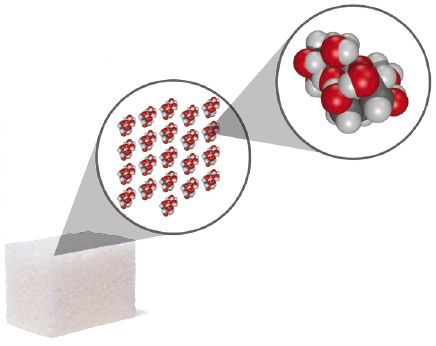
\includegraphics[width=0.35\textwidth]{azucar.jpg}
  \captionof{figure}{\footnotesize Un cubo de azúcar esta constituido por miles de millones
    de moléculas de sacarosa, cada una de ellas con 45 átomos (C$_{12}$H$_{22}$O$_{11}$) .}
  \label{fig:azucar}
\end{wrapfigure}

Los átomos de elementos no metálicos se pueden unir para formar moléculas pequeñas,
como las de agua (H$_2$O) y dióxido de carbono (CO$_2$), pero también pueden formar moléculas con
decenas o centenas de átomos cada una. Considera, por ejemplo, los casos del octano (C$_8$H$_{18}$),
el componente principal de la gasolina, en el que cada molécula está compuesta por 26 átomos,
o el azúcar (también llamada sacarosa, C$_{12}$H$_{22}$O$_{11}$), con 45 átomos por molécula (figura \ref{fig:azucar}).

En nuestro mundo, una gran proporción de las sustancias naturales y sintéticas resulta de la
combinación de los siguientes elementos no metálicos: carbono (C), hidrógeno (H), oxígeno (O), nitrógeno
(N) y azufre (S). Veamos algunos ejemplos en la siguiente actividad.

\begin{minipage}{\textwidth}
  \begin{boxK}
    Investiga y comunica
    \begin{enumerate}
      \item Investiga la fórmula condensada y estructural de las moléculas que constituyen las siguientes sustancias.
            \begin{enumerate}
              \item Cafeína: sustancia estimulante en bebidas como el café y los refrescos.
              \item Capsaicina: sustancia que causa la sensación picante de los chiles.
              \item Alicina: sustancia responsable del olor del ajo.
            \end{enumerate}
      \item Determina de qué tipos y de cuántos átomos en total se conforma cada molécula, y qué tipos de enlaces
            (sencillos, dobles, o triples) establecen.
      \item Comparte los resultados de tu investigación con tus compañeros y verifíquenlos.
    \end{enumerate}
  \end{boxK}
\end{minipage}

\subsubsection{Sustancias metálicas}

\begin{figure}[H]
  \centering
  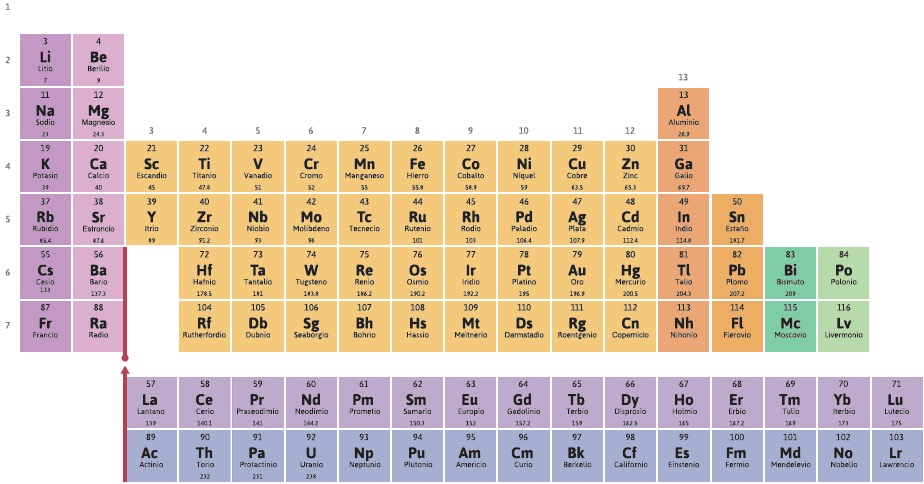
\includegraphics[width=\textwidth]{metales.jpg}
  \captionof{figure}{\footnotesize Elementos metálicos.}
  \label{fig:metales}
\end{figure}

\begin{wrapfigure}{r}{0.5\textwidth}
  \centering
  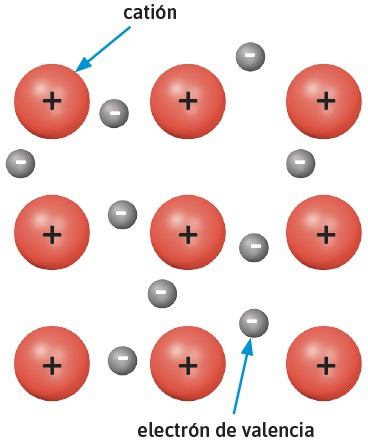
\includegraphics[width=0.28\textwidth]{electron_valencia.jpg}
  \captionof{figure}{\footnotesize Representación del modelo de \emph{mar de electrones} para un metal.}
  \label{fig:electron_valencia}
\end{wrapfigure}

La mayoría de los elementos químicos en la tabla periódica son metálicos
(figura \ref{fig:metales}), cuyos átomos pierden sus electrones con relativa facilidad cuando interaccionan
entre sí o con otro tipo de átomos. Imagina que varios átomos de sodio (Na), un elemento metálico, interaccionan
unos con otros. Durante la interacción cada átomo pierde un electrón de valencia y forma un ion Na+; sin embargo,
los electrones de valencia no se transfieren de forma directa a otros átomos, sino que permanecen moviéndose alrededor
de todos los iones de sodio formados. Por ello se dice que se origina un \emph{mar de electrones}, en el
que los electrones de valencia se desplazan entre todos los iones del sistema (figura \ref{fig:electron_valencia}).
También hay que mencionar que los cationes y electrones permanecen unidos porque unos a otros se atraen debido a
su carga eléctrica, creando una \emph{red metálica}.


\begin{figure}[H]
  \centering
  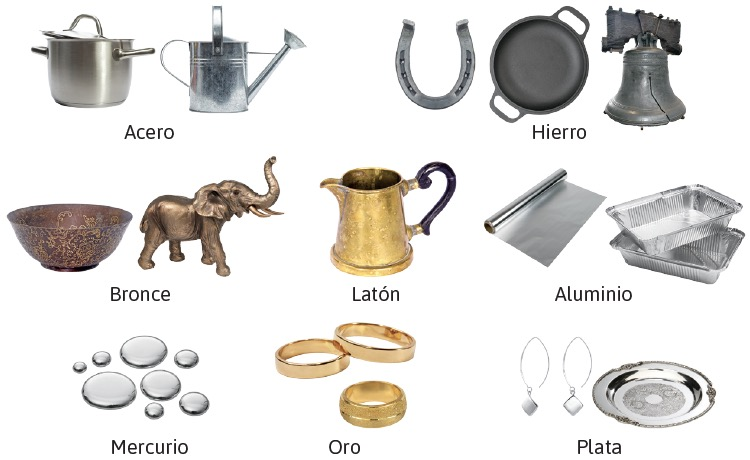
\includegraphics[width=0.6\textwidth]{metalicas.jpg}
  \captionof{figure}{\footnotesize Diferentes tipos de sustancias metálicas.}
  \label{fig:metalicas}
\end{figure}

Como los electrones que forman el \emph{mar} se mueven con facilidad de un lado a otro, los metales
son buenos conductores de corriente eléctrica (esta corriente eléctrica es tan sólo el movimiento de
los electrones de valencia de un lugar a otro en el metal cuando en sus extremos se aplica una
diferencia de voltaje). El mar de electrones también permite que los metales sean buenos conductores
del calor, reflejen la luz y sean maleables (se puedan moldear sin romperse y hacer láminas).
La mayoría de los metales son sólidos a temperatura ambiente, aunque hay sustancias metálicas
líquidas, como el mercurio (Hg) (figura \ref{fig:metalicas}).

\begin{wrapfigure}{r}{0.4\textwidth}
  \centering
  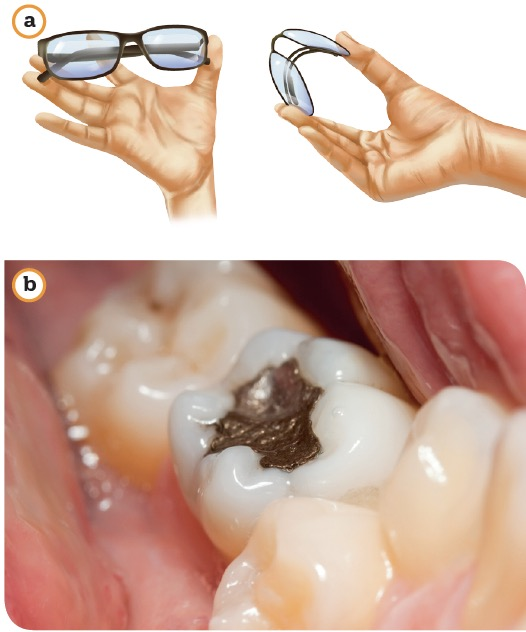
\includegraphics[width=0.4\textwidth]{metalicas2.jpg}
  \captionof{figure}{\footnotesize Diferentes tipos de sustancias metálicas.}
  \label{fig:metalicas2}
\end{wrapfigure}

Los metales no forman compuestos químicos cuando se combinan con otros metales, tan sólo se mezclan.
Estas mezclas se llaman aleaciones, y los químicos e ingenieros en materiales han logrado
hacer mezclas metálicas con propiedades extraordinarias. La mayoría de los materiales metálicos
que cada día usamos está hecha de aleaciones, como el acero, el bronce, la alpaca, el peltre y
las amalgamas. Algunas de ellas tienen propiedades superplásticas, esto es, pueden estirarse
hasta alcanzar cien veces su longitud original sin romperse. Un ejemplo es la amalgama de zinalco,
una aleación de cinc (Zn) y aluminio (Al). Otras como el nitinol formado por la mezcla de níquel (Ni)
y titanio (Ti), originan materiales que recuperan su forma original después de deformarlos (figura \ref{fig:metalicas2}).

\begin{wrapfigure}{l}{0.3\textwidth}
  \centering
  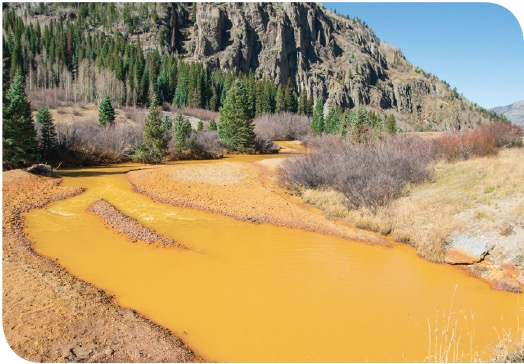
\includegraphics[width=0.3\textwidth]{metalicas3.jpg}
  \captionof{figure}{\footnotesize Contaminación causada durante la extracción de hierro.
    El color rojizo se debe a especies oxidadas de hierro.}
  \label{fig:metalicas3}
\end{wrapfigure}

¿Imaginas tu vida sin materiales metálicos? Sin cobre (Cu) para fabricar los cables que conducen la
electricidad a la que conectas el televisor, sin la lata de aluminio (Al) maleable de tu bebida
favorita, sin el hierro (Fe) resistente pero con la elasticidad necesaria para construir casas y
edificios, sin el litio (Li) y el cadmio (Cd) de las pilas con las que funcionan los aparatos que
utilizas a diario, como en los teléfonos celulares. Sin duda es difícil concebir un mundo sin metales
porque no tendríamos materiales suficientes para sustituirlos.

En la actualidad, cada año se consumen miles de toneladas de diferentes tipos de metales,
dado que las aplicaciones tecnológicas los requieren; sin embargo, se trata de recursos
no renovables, y su extracción y consumo tiene un gran impacto ambiental (figura \ref{fig:metalicas3}).
Por ello, si no modificamos nuestros hábitos y disminuimos el uso excesivo de los materiales metálicos,
llegaremos sin duda a una emergencia metálica.

\begin{boxK}
  Investiga, argumenta y comunica
  \begin{enumerate}
    \item Seleccionen en equipo un material metálico de uso común y averigüen:
          \begin{enumerate}
            \item sus propiedades físicas y químicas más importantes;
            \item la cantidad de ese metal que anualmente se consume en México y en el mundo;
            \item los tipos de impacto ambiental asociados con su extracción, consumo y desecho.
          \end{enumerate}
    \item Propongan estrategias para sustituir, reusar o reciclar el material metálico seleccionado,
          con el fin de reducir su impacto ambiental. Justifiquen sus propuestas.
    \item Compartan en una exposición en grupo los resultados de su investigación.
  \end{enumerate}
\end{boxK}

\begin{minipage}{0.45\textwidth}
  \begin{figure}[H]
    \centering
    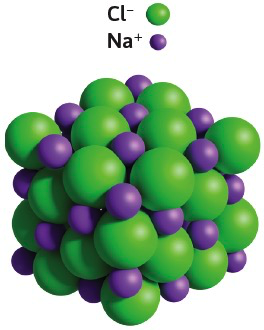
\includegraphics[width=0.5\textwidth]{ionicos1.jpg}
    \captionof{figure}{\footnotesize Representación nanoscópica del cloruro de sodio (NaCl).}
    \label{fig:ionicos1}
  \end{figure}
\end{minipage}\hfill
\begin{minipage}{0.45\textwidth}
  \begin{figure}[H]
    \centering
    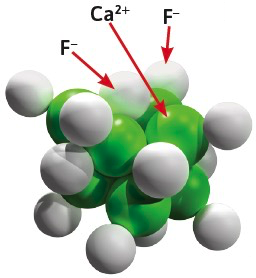
\includegraphics[width=0.5\textwidth]{ionicos2.jpg}
    \captionof{figure}{\footnotesize Representación nanoscópica del fluoruro de calcio (CaF$_2$).}
    \label{fig:ionicos2}
  \end{figure}
\end{minipage}

Los compuestos iónicos, como la sal común (cloruro de sodio, NaCl), resultan de la combinación de
átomos de elementos no metálicos y átomos de elementos metálicos. En general, los átomos de los
elementos metálicos son más grandes que los de elementos no metálicos. Esto causa que los
electrones de valencia de los átomos metálicos estén más alejados del núcleo y se muevan con
más facilidad que los de los no metales. De hecho, cuando átomos de elementos metálicos
interaccionan con los de no metales, los electrones de valencia de los metales se transfieren a
los no metales. En este proceso, los átomos de los metales se transforman en cationes mientras
los de los no metales forman aniones.

Considera, por ejemplo, la interacción entre átomos de sodio (Na, Z = 11, metálico) y de cloro
(Cl, Z = 17, no metálico). En este proceso los átomos de sodio pierden un electrón de valencia
y forman cationes Na$^+$, mientras que los de cloro ganan un electrón de valencia adicional y forman
aniones Cl$^-$. Cuando un trozo de sodio metálico se pone en contacto con una muestra de cloro se
producen millones de iones Na$^+$ y Cl$^-$. Dado que cargas de signos opuestos se atraen, los iones
Na$^+$ y Cl$^-$ forman un conglomerado de iones (red iónica) en el que cada ion está rodeado por iones de signo opuesto (figura 2.25). Esta red es muy estable y el compuesto químico que se forma es el famoso cloruro de sodio, cuya fórmula se representa como NaCl. Es importante destacar que esta fórmula no indica que esta sustancia está constituida por moléculas con un ion de sodio y uno de cloro , sino que en la red tiene miles de iones, y por cada ion de Na+ hay un ion de Cl$^-$.

El mismo modelo se puede utilizar para explicar y predecir la formación de otros compuestos iónicos.
Considera la interacción entre átomos de calcio (Ca, Z = 20, metálico) y de flúor (F, Z = 9, no
metálico). Los átomos de calcio tienden a perder sus dos electrones de valencia cuando interaccionan
con átomos de elementos no metálico como el flúor y, por tanto, se forman cationes Ca2$^+$.
Sin embargo, cada átomo no metálico de flúor sólo es capaz de aceptar un electrón para formar
aniones F$^-$. Como cada átomo de calcio transfiere dos electrones, uno solo de estos átomos
transforma dos de flúor en dos iones fluoruro, F$^-$. Cuando los millones de iones que se generan
interaccionan entre sí, se forma una red iónica en la que hay dos aniones F$^-$ por cada
catión Ca2$^+$. El compuesto iónico que se produce se llama fluoruro de calcio, y su fórmula
condensada es, entonces, CaF$_2$ (en la fórmula el elemento metálico siempre se representa primero)
(figura \ref{fig:ionicos2}).\\

\begin{boxK}
  Infiere, representa e investiga
  \begin{enumerate}
    \item Identifica la fórmula condensada del compuesto iónico que se forma al combinar cada par
          de elementos listados en esta tabla.
          \begin{figure}[H]
            \centering
            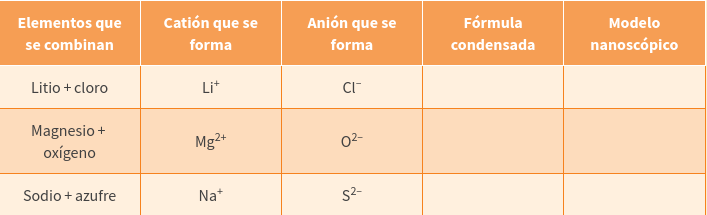
\includegraphics[width=0.8\textwidth]{tabla_ionicos.png}
            \label{fig:tabla_ionicos}
          \end{figure}
    \item Construyan en equipos un modelo de cada compuesto iónico a nivel nanoscópico. Representen la proporción de cada ion en la red iónica.
    \item Investiguen los usos comunes de los compuestos iónicos que se forman.
  \end{enumerate}
\end{boxK}

En general, la fuerza de atracción que mantiene unidos a los iones en compuestos iónicos es grande,
lo cual hace que no se separen con facilidad. Es por ello que estos compuestos tienden a ser sólidos
con altos puntos de fusión, pues es necesario proporcionar gran cantidad de energía para que los
iones se separen y adquieran movilidad.

\begin{boxK}
  \begin{enumerate}
    \item  Analiza el modelo y úsalo para explicar que los compuestos iónicos son sólidos y que se fragmentan con facilidad al golpearlos.
          \begin{figure}[H]
            \centering
            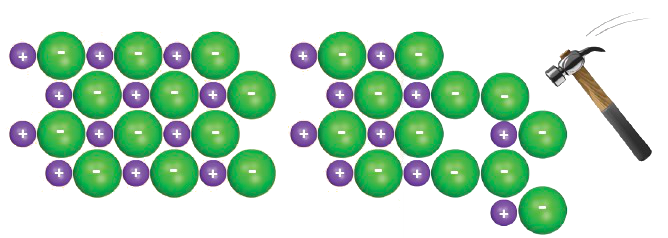
\includegraphics[width=0.6\textwidth]{ionicos3.png}
            \label{fig:ionicos3}
          \end{figure}
    \item Comenta tus ideas con tus compañeros y corríjanlas en caso de ser necesario.
  \end{enumerate}
\end{boxK}

\begin{boxK}
  \begin{enumerate}
    \item Analiza cada representación de distintas sustancias y determina qué tipo de sustancia (molecular, metálica o iónica) se busca representar.
          \begin{figure}[H]
            \centering
            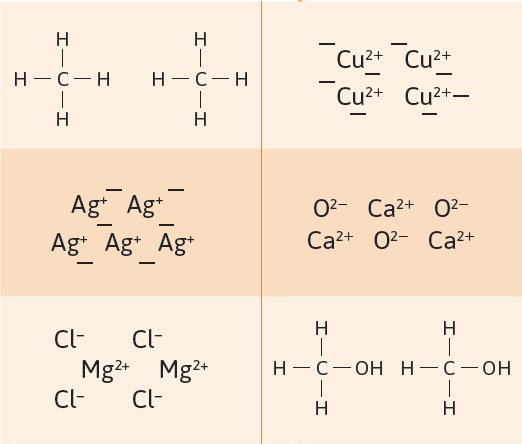
\includegraphics[width=0.6\textwidth]{formulas_condensadas.jpg}
          \end{figure}
    \item Escribe la fórmula condensada de cada una.
    \item Predice las propiedades físicas de esas sustancias, luego investígalas en libros e internet y contrástalas con tus predicciones.
    \item Haz una representación similar a las anteriores de tres sustancias de la actividad del inicio de esta lección y menciona a qué tipo de sustancia corresponde cada grupo que se incluyó en la tabla.
    \item Comparte tus predicciones con tus compañeros de clase y justifícalas con base en la composición y estructura de las distintas sustancias.
  \end{enumerate}
\end{boxK}

\subsubsection{Ejercicios}

\begin{boxK}
  Relaciona el catión y anión que forman el compuesto:\\

  \begin{minipage}{0.5\textwidth}
    \begin{enumerate}
      \item Cloruro de potasio (KCl)
      \item Óxido de magnesio (MgO)
      \item Sulfuro  de sodio (Na2S)
      \item Yoduro de potasio (Kl)
      \item Bromuro de potasio (KBr)
      \item Óxido de hierro (FeO)
      \item Cloruro de potasio  (KCl)
      \item Óxido de calcio (CaO)
      \item Fluoruro de litio (LiF)
      \item Cloruro de berilio (BeCl$_2$)
      \item Fluoruro de sodio (NaF)
      \item Óxido de bario (BaO)
      \item Yoduro de rubidio (Rbl)
      \item Sulfuro de aluminio (Al$_2$S$_3$)
      \item Bromuro de sodio (NaBr)
    \end{enumerate}
  \end{minipage}%
  % \vspace{2cm}
  \begin{minipage}{0.5\textwidth}
    \begin{itemize}
      \item[\rule{1cm}{0.2mm}] Ca$^{2+}$O$^{2-}$
      \item[\rule{1cm}{0.2mm}] K$^+$Br$^-$
      \item[\rule{1cm}{0.2mm}] Mg$^{2+}$O$^{2-}$
      \item[\rule{1cm}{0.2mm}] Fe$^{2+}$O$^{2-}$
      \item[\rule{1cm}{0.2mm}] K$^+$I$^-$
      \item[\rule{1cm}{0.2mm}] K$^+$Cl$^-$
      \item[\rule{1cm}{0.2mm}] K$^+$Cl$^-$
      \item[\rule{1cm}{0.2mm}] Na$^+$S$^{2-}$
      \item[\rule{1cm}{0.2mm}] Ba$^{2+}$+O$^{2-}$
      \item[\rule{1cm}{0.2mm}] Al$^{3+}$S$^{2-}$
      \item[\rule{1cm}{0.2mm}] Be$^{2+}$+Cl$^{-}$
      \item[\rule{1cm}{0.2mm}] Na$^+$Br$^-$
      \item[\rule{1cm}{0.2mm}] Rb$^+$I$^-$
      \item[\rule{1cm}{0.2mm}] Li$^+$F$^-$
      \item[\rule{1cm}{0.2mm}] Na$^+$F$^-$
    \end{itemize}
  \end{minipage}
\end{boxK}

\begin{boxK}
  Relaciona cada elemento con las características que le corresponden.

  \begin{minipage}{0.6\textwidth}
    \begin{enumerate}\footnotesize
      \item Elemento del grupo VII, con siete electrones en la última capa de valencia, ubicado en el tercer periodo de la tabla periódica.
      \item Elemento metaloide, ubicado en el tercer periodo de la tabla periódica.
      \item Elemento conocido como gas noble.
      \item Elemento metálico con Z = 11.
      \item Elemento que se ubica en el grupo 15 y en el periodo 2 de la tabla periódica.
      \item Elemento con 12 protones y 12 electrones.
      \item Elemento no metálico con Z =34
      \item Ejemplo de gas inerte.
    \end{enumerate}
  \end{minipage}\hfill
  \begin{minipage}{0.25\textwidth}
    \begin{itemize}
      \item[\rule{1cm}{0.2mm}] Selenio
      \item[\rule{1cm}{0.2mm}] Neón
      \item[\rule{1cm}{0.2mm}] Magnesio
      \item[\rule{1cm}{0.2mm}] Xenón
      \item[\rule{1cm}{0.2mm}] Sodio
      \item[\rule{1cm}{0.2mm}] Cloro
      \item[\rule{1cm}{0.2mm}] Nitrógeno
      \item[\rule{1cm}{0.2mm}] Silicio
    \end{itemize}
  \end{minipage}
\end{boxK}
\begin{boxK}
  Relaciona cada elemento con las características que le corresponden.

  \begin{minipage}{0.6\textwidth}
    \begin{enumerate}\footnotesize
      \item Elemento con cuatro electrones en su última capa de valencia.
      \item Ejemplo de gas noble.
      \item Elemento de la familia de metales alcalinos.
      \item Metal brillante utilizado en joyería.
      \item Líquido rojo oscuro.
      \item Gas incoloro que arde en presencia de oxígeno.
      \item Metal reactivo que reacciona fácilmente con agua.
    \end{enumerate}
  \end{minipage}\hfill
  \begin{minipage}{0.25\textwidth}
    \begin{itemize}
      \item[\rule{1cm}{0.2mm}] Neón
      \item[\rule{1cm}{0.2mm}] Bromo
      \item[\rule{1cm}{0.2mm}] Calcio
      \item[\rule{1cm}{0.2mm}] Oro
      \item[\rule{1cm}{0.2mm}] Rubidio
      \item[\rule{1cm}{0.2mm}] Hidrógeno
      \item[\rule{1cm}{0.2mm}] Carbono
    \end{itemize}
  \end{minipage}
\end{boxK}

% \begin{boxK}  Relaciona los siguientes elementos:\\
%   \begin{minipage}{0.5\textwidth}
%     \begin{enumerate}

%     \end{enumerate}
%   \end{minipage}%
%   \begin{minipage}{0.5\textwidth}
%     \begin{itemize}

%     \end{itemize}
%   \end{minipage}
% \end{boxK}

\newpage \thispagestyle{plain}
\section{Moléculas de importancia para la vida}
\boxabstract{
  \begin{itemize}
    \item Identifica componentes químicos importantes
          (carbohidratos, lípidos, proteínas, ADN) que participan en
          la estructura y funciones del cuerpo humano.
    \item Representa y diferencia mediante esquemas, modelos y
          simbología química, elementos y compuestos, así como
          átomos y moléculas.
    \item Explica y predice propiedades físicas de los materiales
          con base en modelos submicroscópicos sobre la
          estructura de átomos, moléculas o iones, y sus
          interacciones electrostáticas.
  \end{itemize}
}
\subsection{¿Qué moléculas nos constituyen?}

\newpage \thispagestyle{plain}
\section{Relaciones entre la estructura y las propiedades de las sustancias}
\boxabstract{
  \begin{itemize}
    \item Representa y diferencia mediante esquemas, modelos y
          simbología química, elementos y compuestos, así como
          átomos y moléculas.
    \item Explica y predice propiedades físicas de los materiales
          con base en modelos submicroscópicos sobre la
          estructura de átomos, moléculas o iones, y sus
          interacciones electrostáticas.
  \end{itemize}
}
\subsection{¿Cómo interaccionan las moléculas?}
\subsection{¿Cómo se explican y predicen las propiedades de las sustancias?}



% \newpage \thispagestyle{plain}
% \section{Reacciones químicas en nuestro mundo}
% \subsection{¿Cuál es la evidencia de que las sustancias reaccionan unas con otras?}

% \newpage \thispagestyle{plain}
% \section{Recombinaciones atómicas}
% \subsection{¿Cómo representamos las reacciones qu\'imicas?}
% \subsection{¿Qué cambia y qué se conserva durante las reacciones químicas?}

% \newpage \thispagestyle{plain}
% \section{Cantidad de las sustancias}
% \subsection{¿Cómo determinamos la cantidad de las sustancias?}
% \subsection{Cantidad de las sustancias en reacciones químicas}

% \newpage
% \chapter{}

% \newpage \thispagestyle{plain}
% \section{Un mundo de reacciones químicas}
% \subsection{¿Cómo nos afectan las reacciones químicas?}
% \subsection{¿Cómo aprovechamos las reacciones químicas?}

% \newpage \thispagestyle{plain}
% \section{Energía y reacción química}
% \subsection{¿Cómo se transfiere energía durante las reacciones químicas?}
% \subsection{¿Por qué se transfiere energía durante las reacciones químicas?}

% \newpage \thispagestyle{plain}
% \section{La energía química en nuestras vidas}
% \subsection{¿Cuáles son los beneficios, costos y riesgos de usar energía química?}

% \newpage \thispagestyle{plain}
% \section{Aporte calórico de los alimentos}
% \subsection{¿De dónde proviene la energía que necesitamos para vivir?}

% \newpage \thispagestyle{plain}
% \section{Rapidez de reacción}
% \subsection{¿Qué factores afectan la rapidez de las reacciones químicas?}

% \newpage \thispagestyle{plain}
% \section{La rapidez de reacción y el modelo cinético de partículas}
% \subsection{¿Cómo explicamos diferencias en la velocidad de reacción?}

% \newpage \thispagestyle{plain}
% \section{Utilidad de controlar la rapidez de las reacciones}
% \subsection{¿Cómo controlamos y aprovechamos la velocidad de reacción?}

\end{document}